\section{pre-DC1}

As part of my PhD work, I led the analysis of pre-DC1, a modified version of the \textsc{Lemaître} DC1 in which the supernova light curves 
are generated using a SALT model that satisfies the NaCl constraints. This ensures that the simulations are self-consistent with the model 
assumptions used in the analysis, allowing us to isolate potential biases introduced by the pipeline itself, rather than those arising 
from a mismatch between the simulation and the fitted model. Using these self-consistent pre-DC1 simulations, we can assess the accuracy 
of the reconstructed parameters and their uncertainties on \textsc{Lemaître}-like datasets.

\subsection{Simulation step}

All of the elements concerning the generation of the pre-DC1 supernovae can be summarized in the following list: 
\begin{itemize}
    \item All of the supernova data were generated with SkySurvey \footnote{\url{https://github.com/MickaelRigault/skysurvey}}.
    \item The cosmology that was used is Planck18 found in astropy.cosmology ($\Omega_m=0.30966$) (\cite{Planck_2018_params}).
    \item The color and stretch of the supernovae were drawn from a normal distribution centered around 0, with $\sigma(c) = 0.1$ and $\sigma(X_1) = 1$.
    \item There are no redshift errors added to any supernovae.
    \item A spectrum is generated for each supernova from ZTF and SNLS drawn from a phase when the SN was observed.
    \item Magnitude cuts were applied before the application of any noise and intrinsic dispersion. For each survey the magnitude cuts are written in table \ref{tab:mag_cuts}. This ensures that there are no selection effects added to the simulations.
    \item The rate of the supernovae was chosen to be Frohmaier+19 (\cite{Frohmaier_2019}).
    \item The Milky Way dust extinction was drawn from the Planck dust map and the $E(B-V)_{MW}$ values follow the CCM89 dust law (\cite{Cardelli_1989}).
    \item The addition of the intrinsic dispersion, $\sigma_{int}$, is applied on the observed magnitudes of each supernova.
    \item Light curve measurement uncertainties were drawn from sncosmo \footnote{\url{https://sncosmo.readthedocs.io/en/stable/}} as a function of the skynoise taken from the real observational logs.
    \item An error snake is also added to the light curves drawn from a normal distribution with a dispersion of 5\% of the flux. The error snake term is the same for a given band and given night for a given supernova.
\end{itemize}

\begin{table}[ht]
    \centering
    \begin{tabular}{ c  c }
    \hline
        ZTF & 18.3 \\
        \hline
        SNLS & 24.2 \\
        \hline
        HSC & 24.6 \\
    \hline
    \end{tabular}
    \caption{List of the magnitude cuts on DC1 simulations}
    \label{tab:mag_cuts}
\end{table}


\subsection{Goals}

The goal of the pre-DC1 analysis is to assess the consistency of the 
Georges pipeline (see Section \ref{sec:georges}) in reconstructing the input supernova distances and 
cosmological parameters. To this end, the complete analysis chain is applied 
to 100 realizations of the pre-DC1 dataset, which allows us to assess both the 
accuracy of the reconstructed parameters and the validity of their estimated 
uncertainties. 

More specifically, we first verify that the reconstructed supernova 
parameters $X_0$, $X_1$, $c$, and $t_{max}$ are unbiased with respect 
to their input values. The reliability of the parameter uncertainties is 
tested by comparing the uncertainties obtained from the inverse Fisher 
matrix described in Equation \ref{eqn:nacl_cov}, $\sigma_{\text{Fisher}}$, with those derived from the empirical 
covariance matrix measured across the 100 realizations, 
$\sigma_{\text{Emp}}$. We then assess whether the reconstructed distance 
moduli $\mu$ are unbiased. Finally, we test whether the cosmological parameters 
$\Omega_m$ and $w$ are unbiased when the analysis is performed assuming a 
flat $w$CDM cosmology with a constant equation-of-state parameter $w$. 


\section{Results: Potential Biases \& Systematics}
For the pre-DC1 simulations, we deliberately reduce the effective ZTF SN sample to approximately 500 SNe per simulation, corresponding to a 
total sample of $\sim 1500$ supernovae across the simulations. 
The average time it takes to train one pre-DC1 sample of supernovae is $\sim$ 1h30mins on the IN2P3 Computing Cluster\footnote{\url{https://cc.in2p3.fr/en/}}. 
The duration of each step in the training recipe can be summarized in Table \ref{tab:pre_dc_log}\\

\begin{table}[ht]
    \centering
    \begin{tabular}{ l | l }
    \hline
        Step & Time \\
        \hline
        Light curve fitting & $\sim$30 seconds\\
        \hline
        Spectrum recalibration & $\sim$30 seconds\\
        \hline
        Initial model guess & $\sim$1 hour\\
        \hline
        Initial error model guess & $\sim$1 minute\\
        \hline
        Fitting all parameters & $\sim$ 25 minutes \\
    \hline
    \end{tabular}
    \caption{Duration of each step in the training when applied to a pre-DC1 simulation.}
    \label{tab:pre_dc_log}
\end{table}


\subsection{Model \& Data Agreement}

We present the model and data agreement results on a randomly selected 
realization of pre-DC1.

\subsubsection{Photometry}

Figure \ref{fig:dc1_lc_pulls} shows the photometric weighted 
residuals normalized by the measurement uncertainties (pulls) as a function 
of phase. The pulls are centred around zero across the full phase 
range covered by the model, indicating that NaCl describes the 
photometric data without systematic phase-dependent biases. 
Figure \ref{fig:dc1_lc_band_resid} shows the pull distributions 
per band. Each distribution is fitted with a Gaussian that has a standard deviation of 1. 
The fitted means are 
consistent with zero, confirming that the model does not 
introduce band-dependent biases.

To assess whether the description of the data is accurate accross different redshifts, Figure \ref{fig:dc1_lc_chi2} shows 
the local $\chi^2_{\text{SN}}$ evaluated per supernova as a function of 
redshift. 
No redshift-dependent trend is observed, demonstrating 
that NaCl provides a uniform description across the full redshift 
range of the sample. Finally, Figure \ref{fig:dc1_lc_resid} shows 
the stacked local $\chi^2_{\text{loc}}$ calculated for each each photometric observation as a function of both phase and wavelength. 
The description remains accurate throughout the model's domain of 
definition.

\begin{figure}[ht]
    \centering
    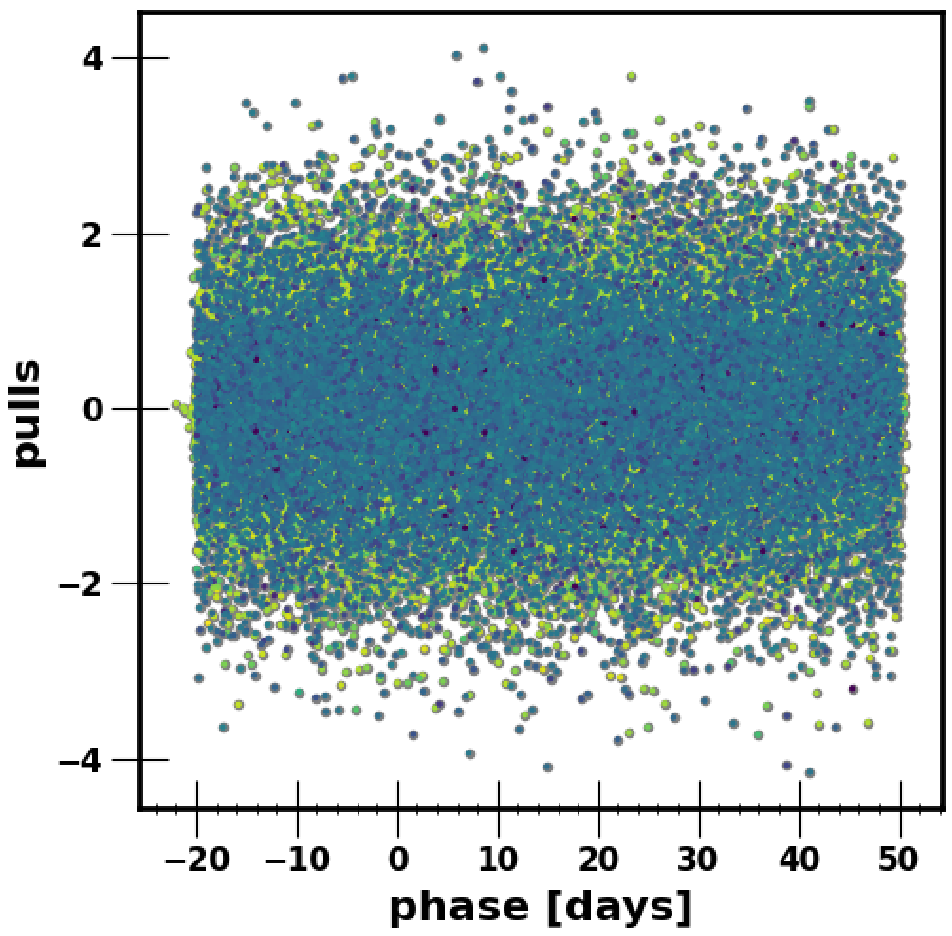
\includegraphics[width=0.5\textwidth]{MainLayout/DC_chapter/figures/new_fig/lc_pulls.png}
    \caption{Photometric pulls as a function of phase for one 
    realization of pre-DC1. The pulls are centred around zero 
    across the full phase range.}
    \label{fig:dc1_lc_pulls}
\end{figure}

\begin{figure}[ht]
    \centering
    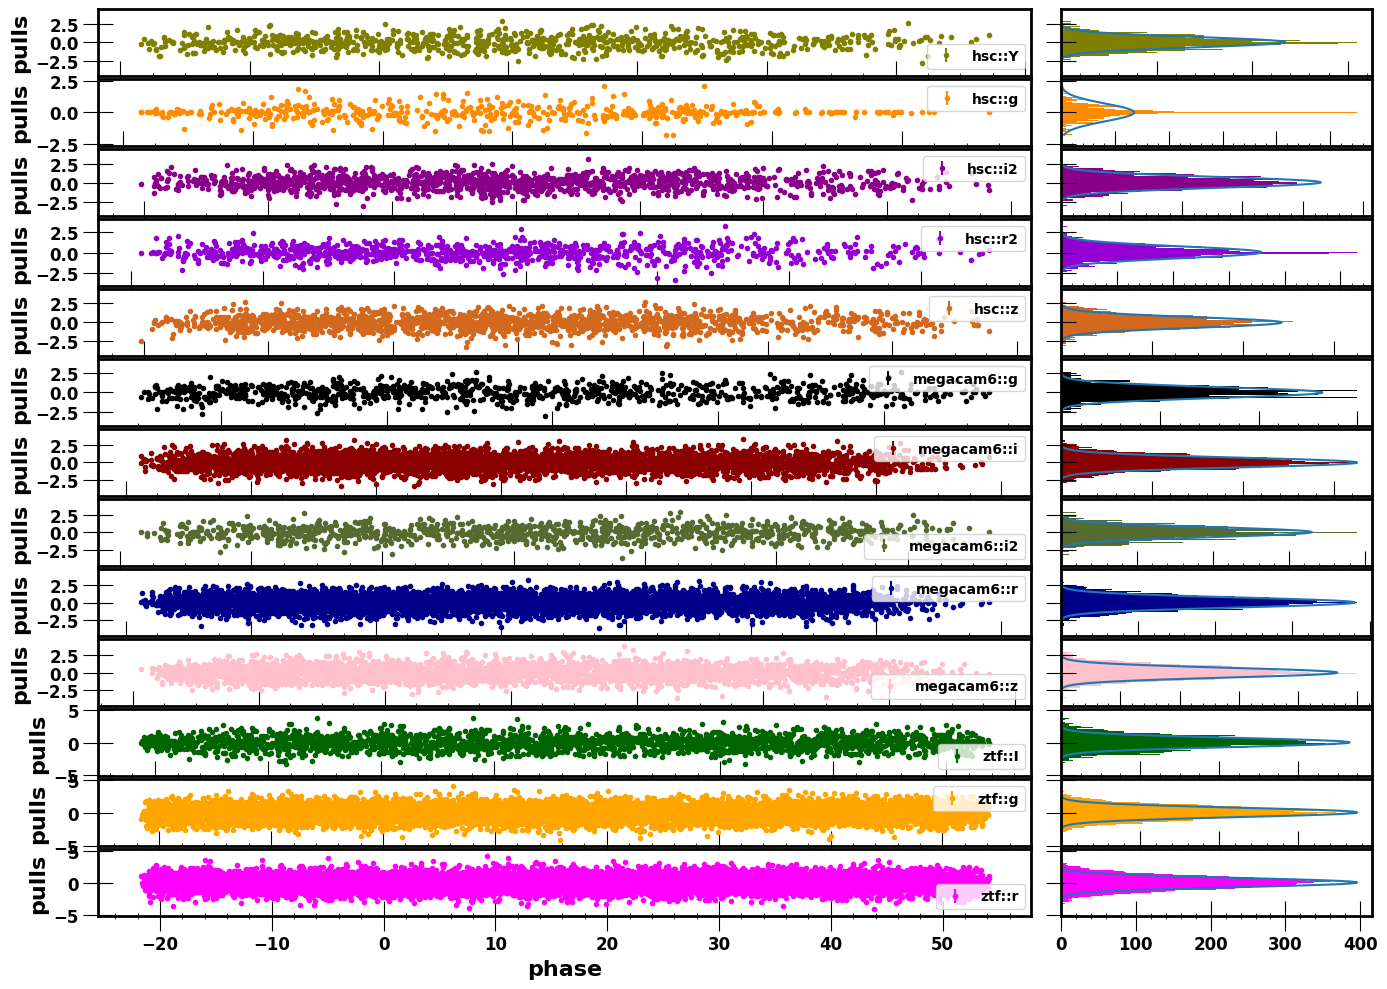
\includegraphics[width=1\textwidth]{MainLayout/DC_chapter/figures/new_fig/lc_pulls_per_band.png}
    \caption{\textit{Left}: Photometric pulls per band for one 
    realization of pre-DC1. \textit{Right}: Histogram of the pulls 
    per band, each fitted with a Gaussian (solid line). The fitted 
    means are consistent with zero.}
    \label{fig:dc1_lc_band_resid}
\end{figure}

\begin{figure}[ht]
    \centering
    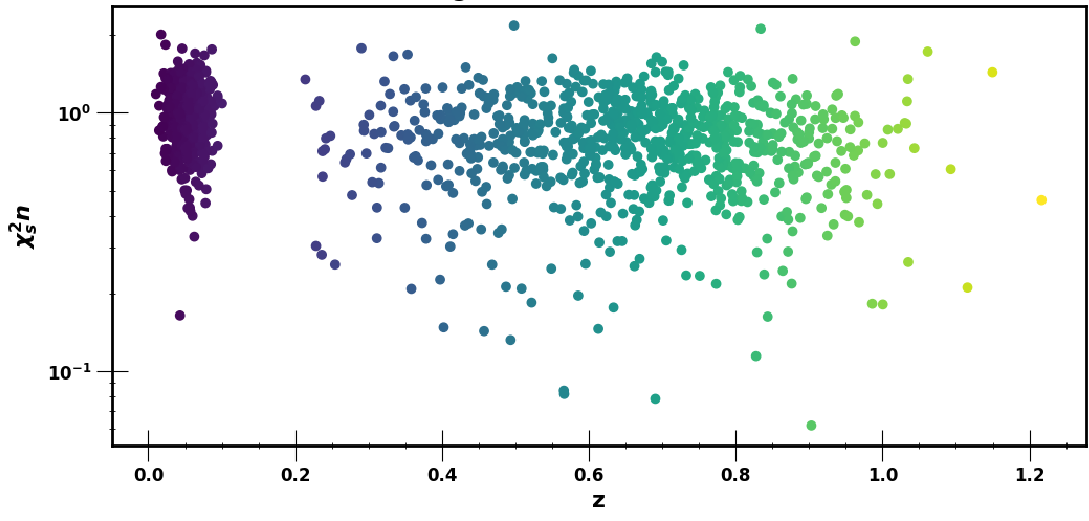
\includegraphics[width=0.8\textwidth]{MainLayout/DC_chapter/figures/new_fig/lc_chi2_z.png}
    \caption{Photometric $\chi^2_{\text{SN}}$ per supernova as a function 
    of redshift for one realization of pre-DC1.}
    \label{fig:dc1_lc_chi2}
\end{figure}

\begin{figure}[ht]
    \centering
    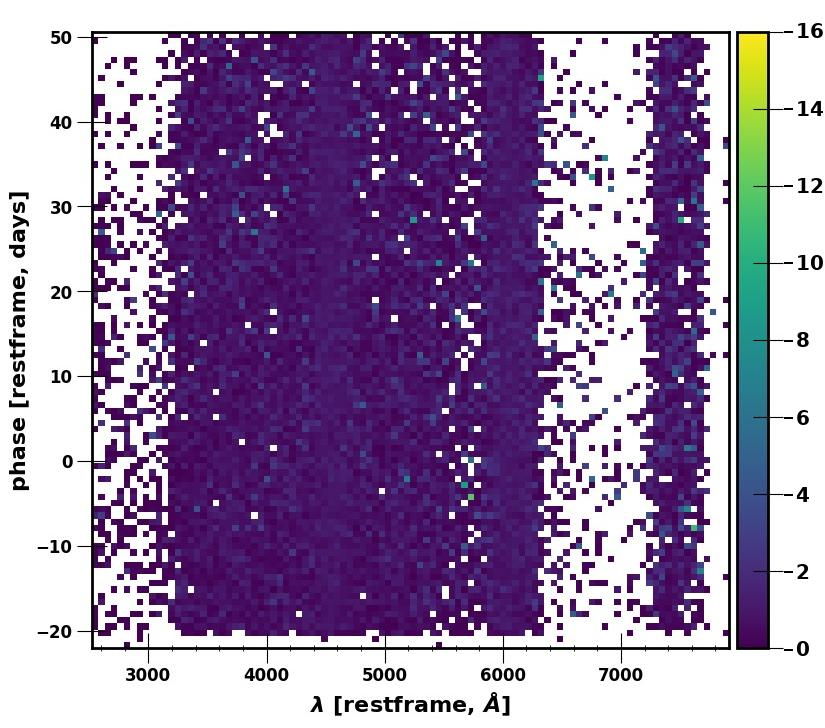
\includegraphics[width=0.8\textwidth]{MainLayout/DC_chapter/figures/new_fig/phot_chi2_edit.jpeg}
    \caption{Stacked photometric $\chi^2_{\text{loc}}$ as a function of phase 
    and wavelength for one realization of pre-DC1.}
    \label{fig:dc1_lc_resid}
\end{figure}

\subsubsection{Spectroscopy}

The spectroscopic analysis yields consistent results. 
Figure 
\ref{fig:dc1_spec_pulls} shows the spectroscopic pulls as a 
function of wavelength. They are centred around zero across 
the full wavelength range. 
Figure \ref{fig:dc1_spec_chi2} shows the supernova $\chi^2_{\text{SN}}$ calculated using the spectroscopic data 
as a function of redshift, which again shows no 
redshift-dependent trend. Figure \ref{fig:dc1_spec_resid} 
shows the stacked $\chi^2_{\text{loc}}$ over wavelength confirming a 
uniformly accurate spectroscopic description.

\begin{figure}[ht]
    \centering
    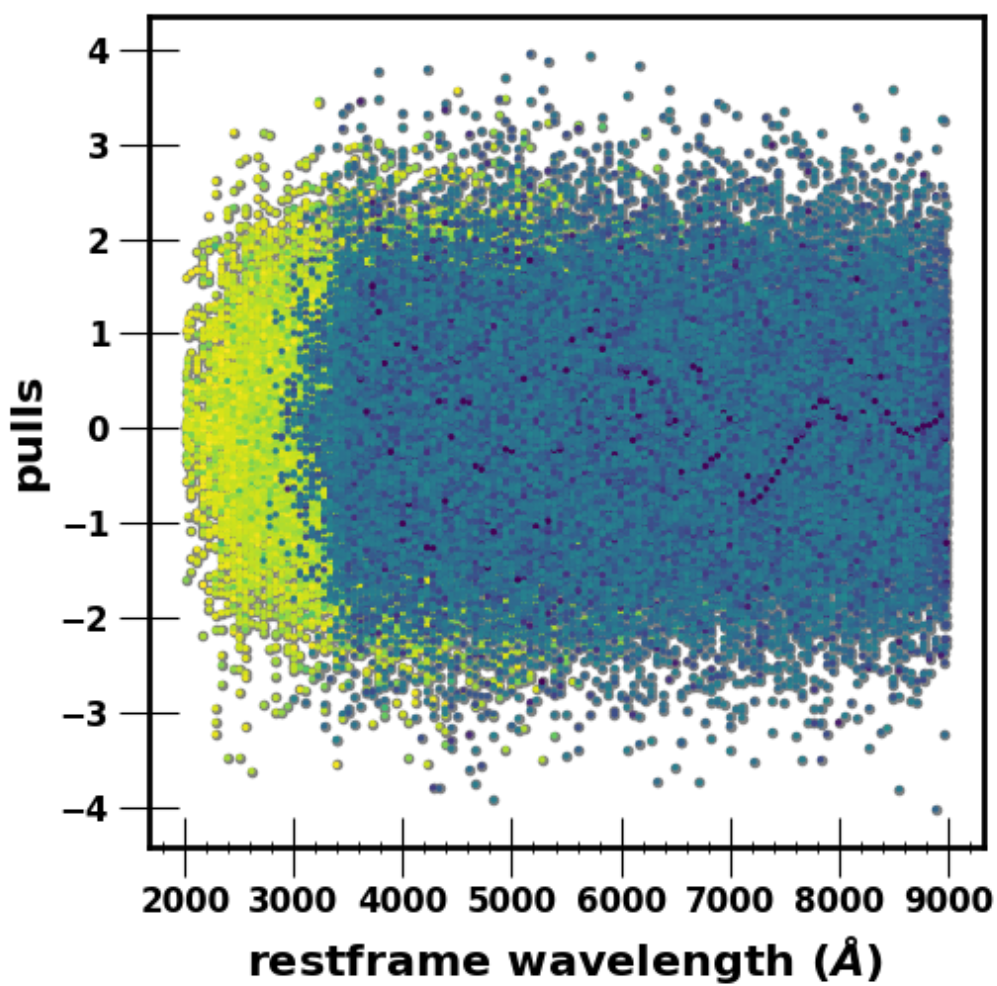
\includegraphics[width=0.5\textwidth]{MainLayout/DC_chapter/figures/new_fig/spec_pulls.png}
    \caption{Spectroscopic pulls as a function of wavelength for 
    one realization of pre-DC1.}
    \label{fig:dc1_spec_pulls}
\end{figure}

\begin{figure}[ht]
    \centering
    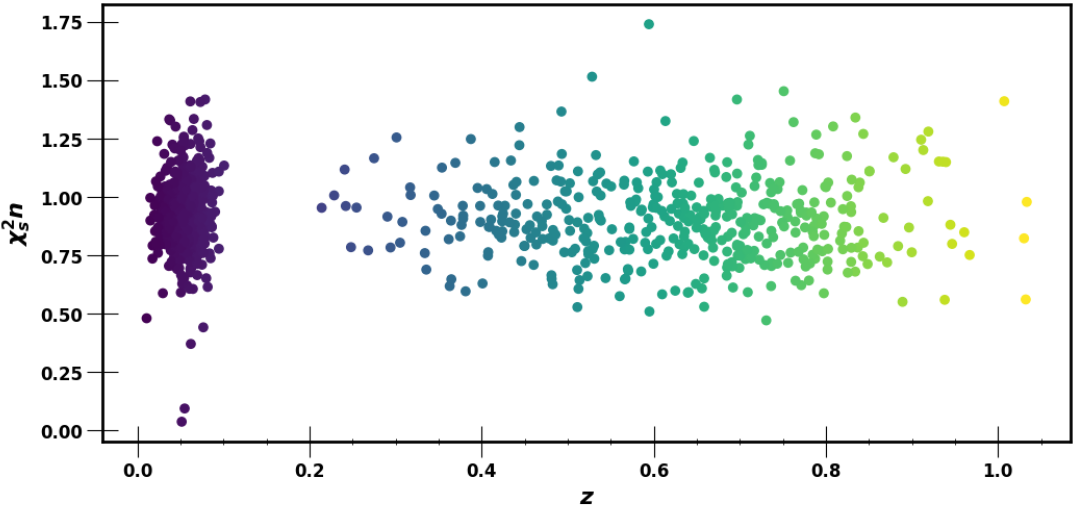
\includegraphics[width=0.8\textwidth]{MainLayout/DC_chapter/figures/new_fig/spec_chi2_z.png}
    \caption{Spectroscopic $\chi^2$ per supernova as a 
    function of redshift for one realization of pre-DC1.}
    \label{fig:dc1_spec_chi2}
\end{figure}

\begin{figure}[ht]
    \centering
    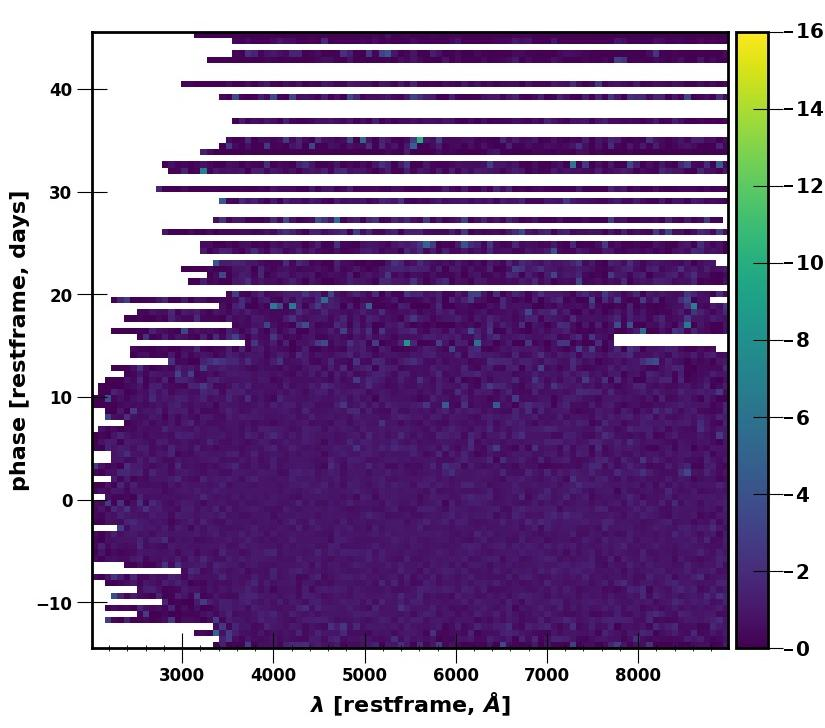
\includegraphics[width=0.8\textwidth]{MainLayout/DC_chapter/figures/new_fig/spec_chi2_edit.jpeg}
    \caption{Stacked spectroscopic $\chi^2$ as a function of 
    wavelength for one realization of pre-DC1.}
    \label{fig:dc1_spec_resid}
\end{figure}



\subsection{Parameter Reconstruction and Covariance Matrix}

Since the pre-DC1 dataset is generated with a model that respects NaCl constraints, we expect to reconstruct the exact same parameters used in the generation. 
In Figure \ref{fig:sn_pars_wres} we compare the generated and reconstructed $X_0$, $X_1$, $c$ and $t_{max}$ parameters averaged over all 100 realizations of pre-DC1. 
This is done by calculating the pulls for each parameter. This is observed as a function of redshift 
to verify whether NaCl introduces redshift-dependent biases on the supernova parameters. 
We see that the reconstructed parameters match the input parameters within the statistical uncertainties of the reconstruction.\\

\begin{figure}[ht]
    \centering
    %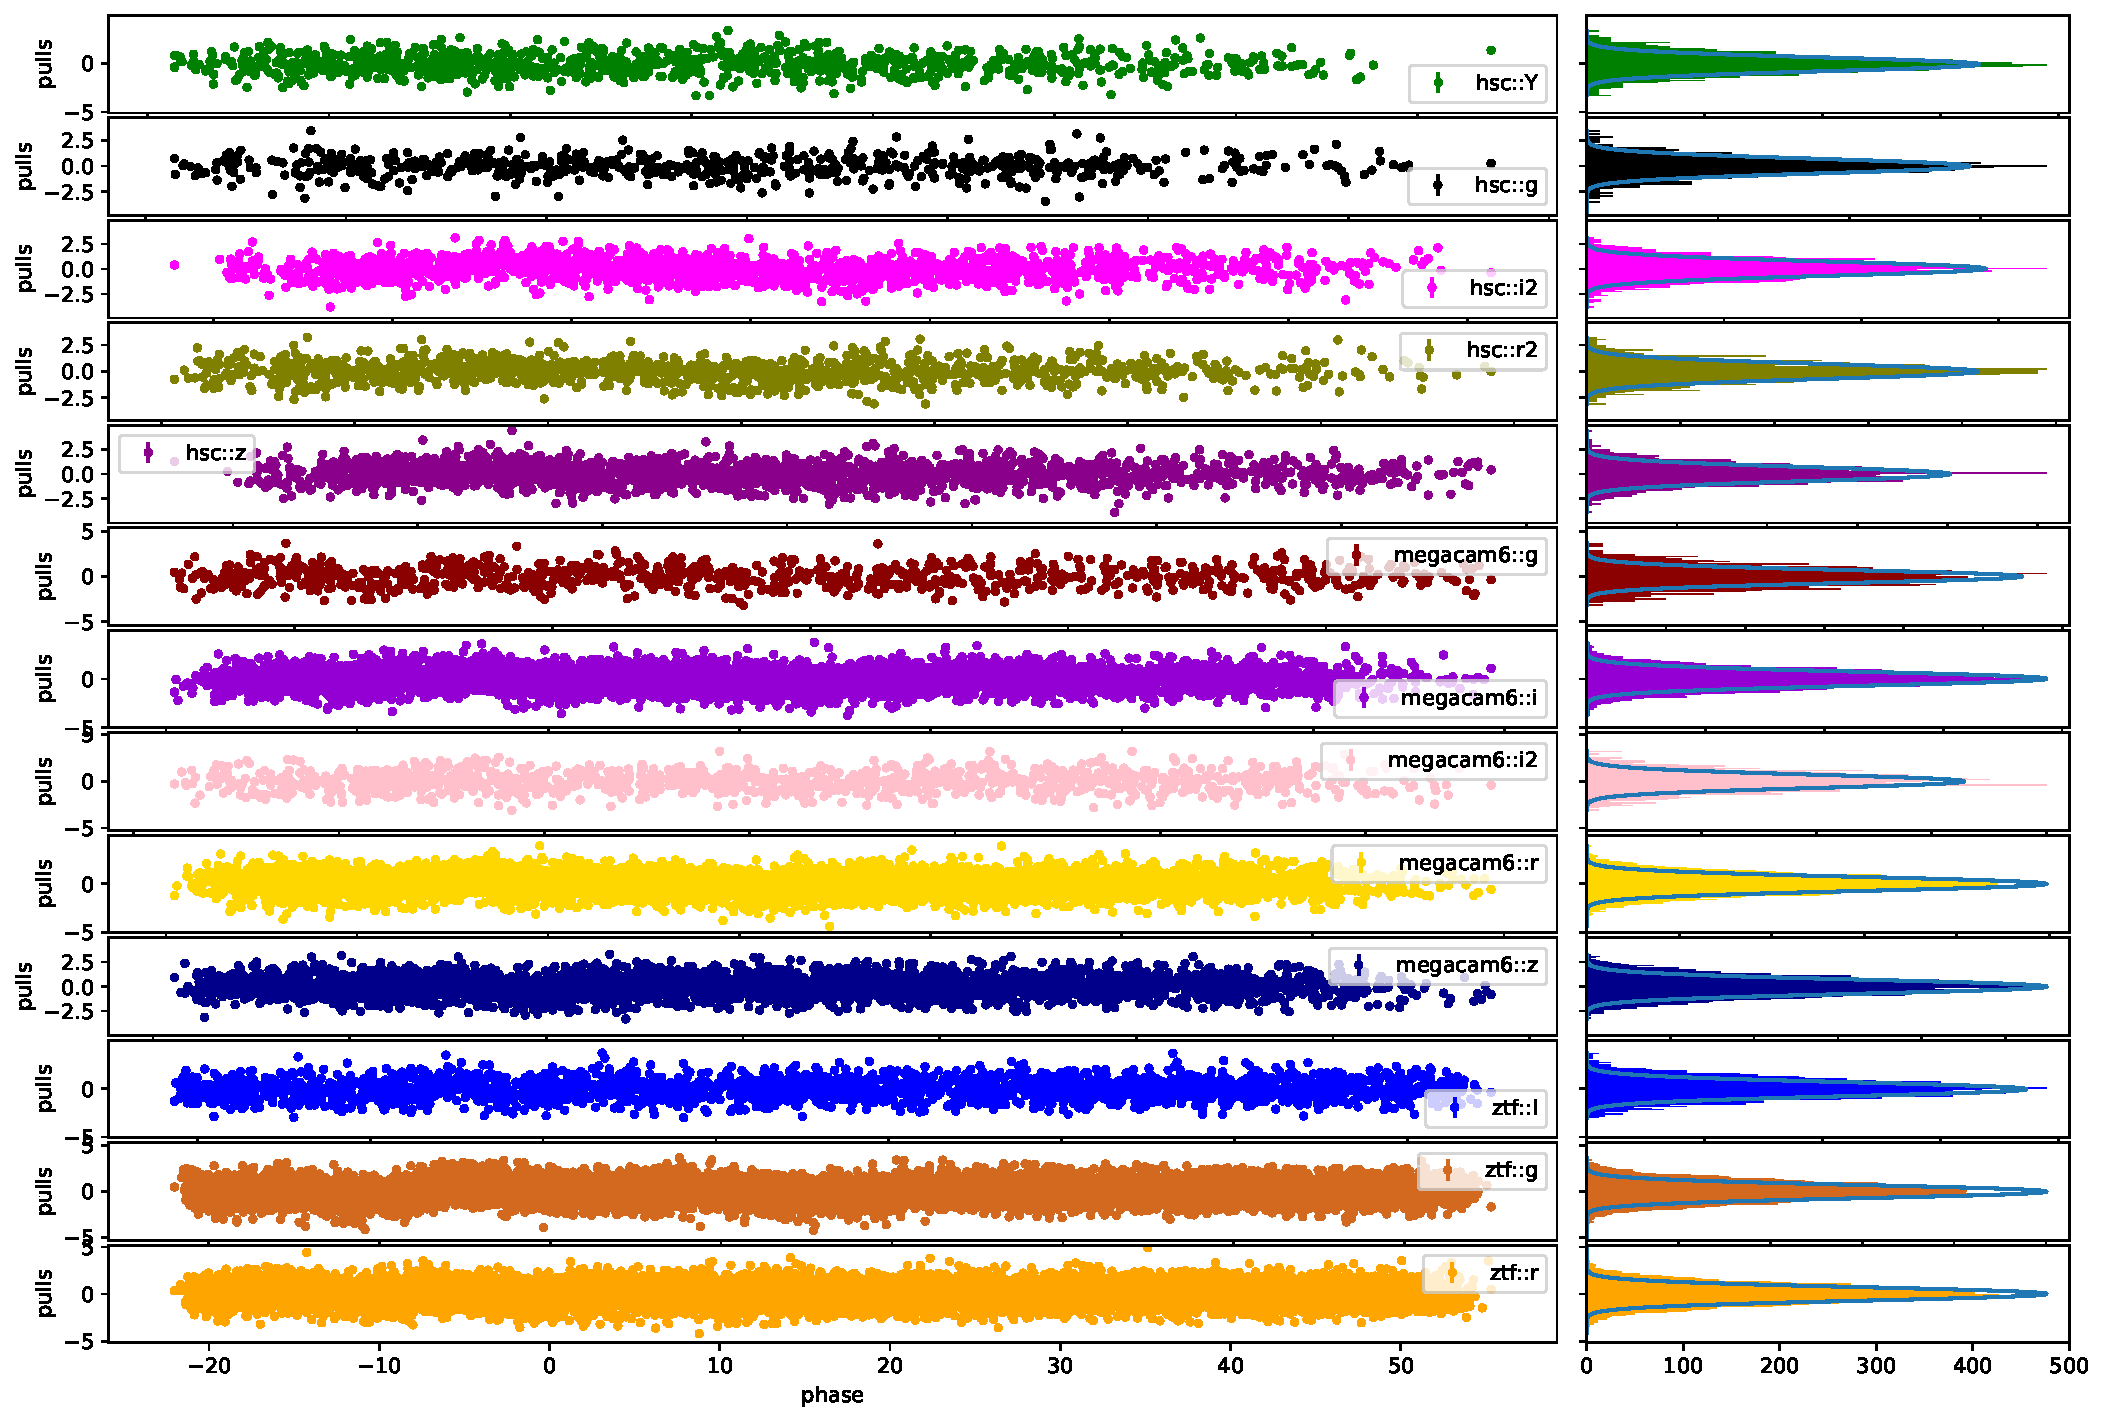
\includegraphics[width=1\textwidth]{MainLayout/DC_chapter/figures/band_resid.pdf}
    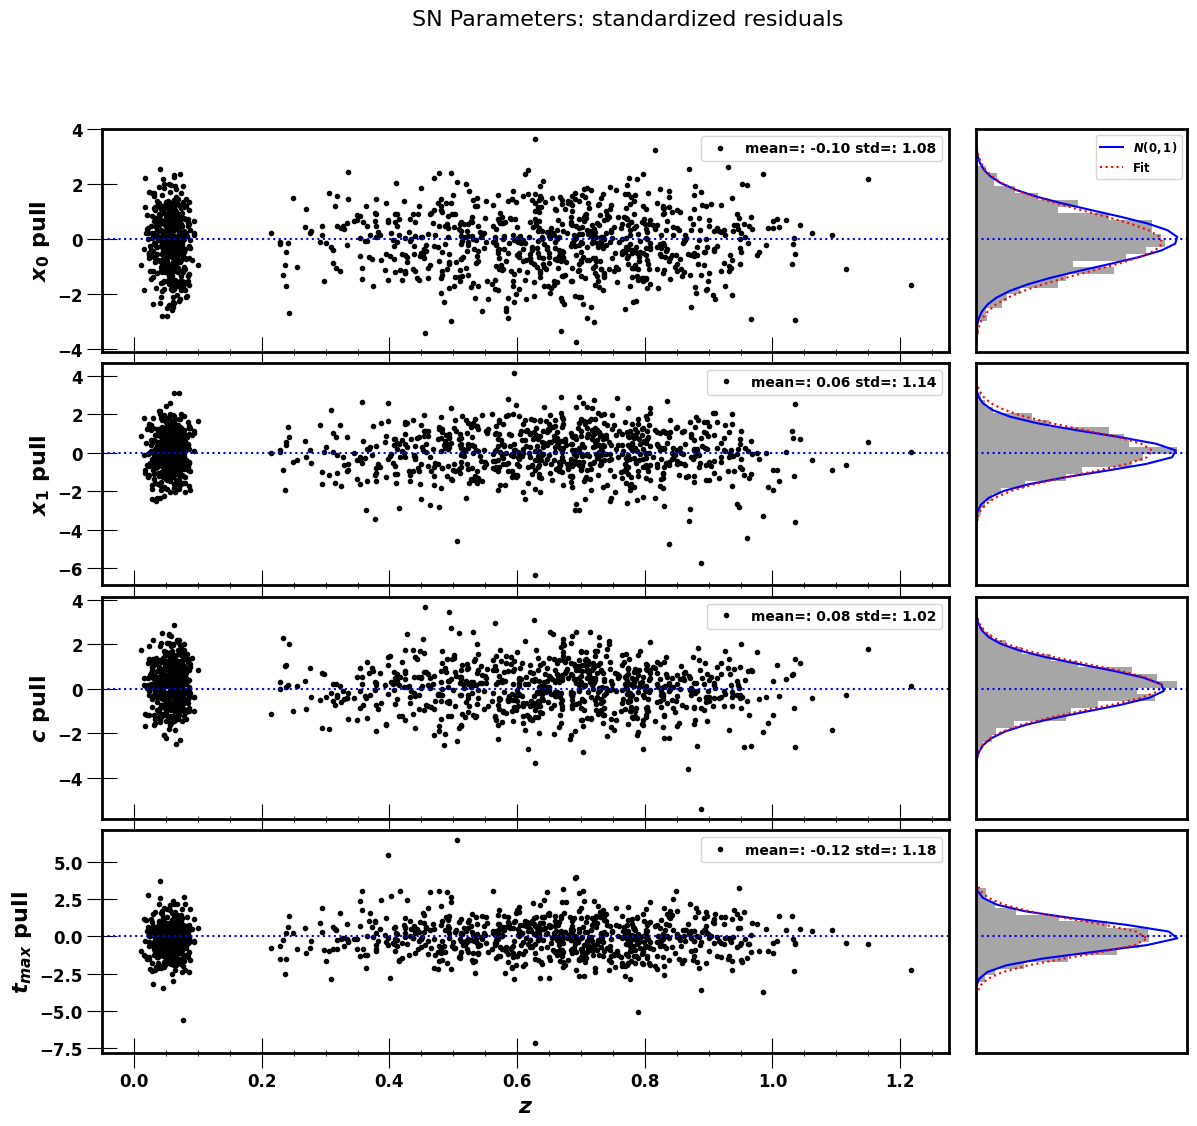
\includegraphics[width=1\textwidth]{MainLayout/DC_chapter/figures/new_fig/sn_pars_wres.png}
    \caption{Weighted residuals of each supernova parameter for 100 realizations of pre-DC1}
    \label{fig:sn_pars_wres}
\end{figure}

We are also interested in comparing the constructed empirical covariance matrix and the Fisher covariance matrix from NaCl. In Figure \ref{fig:pars_cov}, we compare the 
output uncertainties $\sigma_{\text{Fisher}}$ from one pre-DC1 realization with the uncertainties extracted from the empirical uncertainties $\sigma_{\text{Emp}}$ constructed from the run 
on the 100 pre-DC1 realizations as a function of redshift. A more visual representation can be seen in Figure \ref{fig:pars_corr} where compare the correlation matrices constructed from the 
Fisher covariance matrix and the empirical covariance matrix. 
We calculate the ratio of $\sigma_{\text{Emp}}$/$\sigma_{\text{Fisher}}$ and we see that for large part the uncertainties 
are near 1 with a preference for the empirical uncertainties to be slightly higher than the uncertainties predicted by the NaCl output. This likely due to the fact that 
100 realizations may not be enough to reconstruct an exact covariance matrix. 
To assess whether 100 realizations are sufficient to estimate the 
empirical covariance, a previous iteration of pre-DC1 with $\sim 1000$ 
supernovae per realization was used to generate 900 realizations. 
Comparing the empirical covariance constructed from 100 vs 900 
realizations showed that the ratio $\sigma_{\text{Emp}}/\sigma_{\text{Fisher}}$ 
converges toward unity with increasing sample size, confirming that 
the residual excess in the 100-realization estimate is a finite-sample 
effect rather than a systematic bias in the NaCl uncertainty 
propagation. The slight overestimate of $\sigma_{\text{Emp}}$ relative 
to $\sigma_{\text{Fisher}}$ seen in Figure \ref{fig:pars_cov} is 
therefore not a cause for concern.


\begin{figure}[ht]
    \centering
    %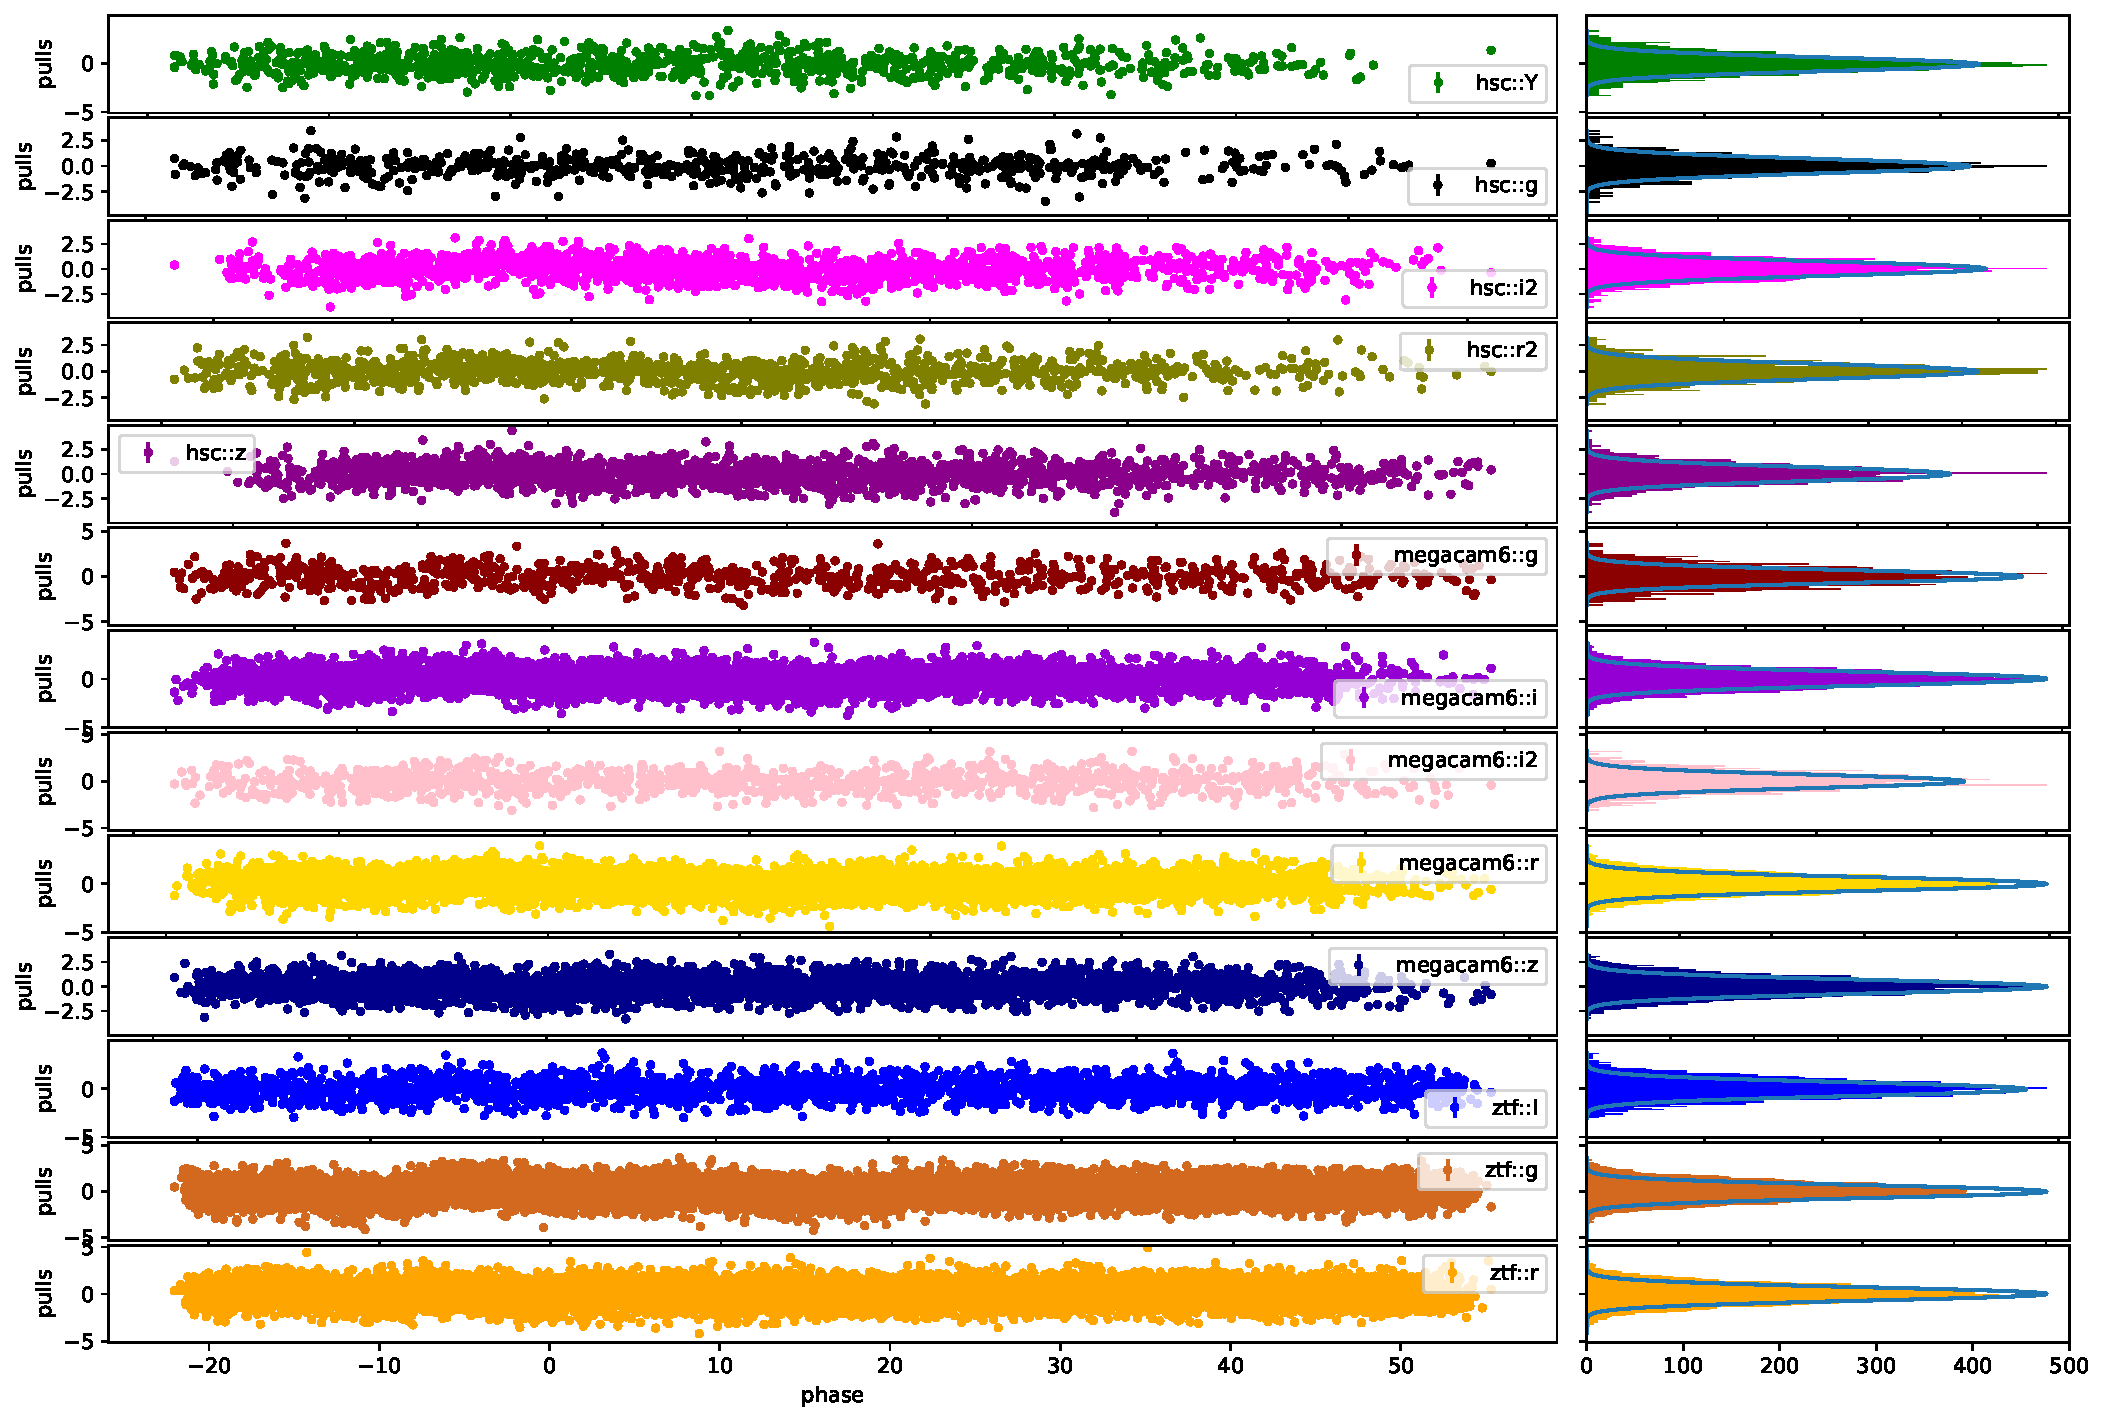
\includegraphics[width=1\textwidth]{MainLayout/DC_chapter/figures/band_resid.pdf}
    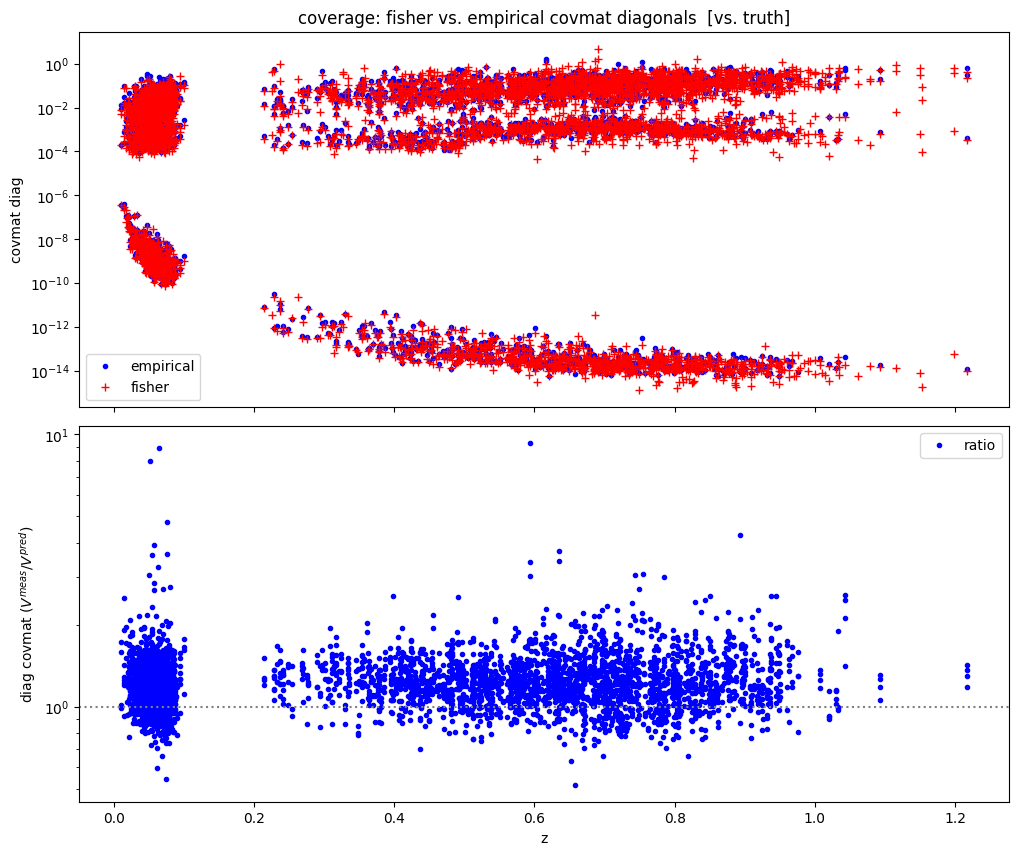
\includegraphics[width=0.8\textwidth]{MainLayout/DC_chapter/figures/new_fig/coverage_all.png}
    \caption{\textit{Top}: $\sigma_{\text{Fisher}}$ in red cross and $\sigma_{\text{Emp}}$ blue dots as a function of redshift. We see distinct layers in the uncertainties that are related 
    to the different parameters $X_0$, $X_1$, $c$ and $t_{max}$. \textit{Bottom}: Ratio of the $\sigma_{\text{Emp}}$ and $\sigma_{\text{Fisher}}$.}
    \label{fig:pars_cov}
\end{figure}


\begin{figure}[ht]
    \centering
    %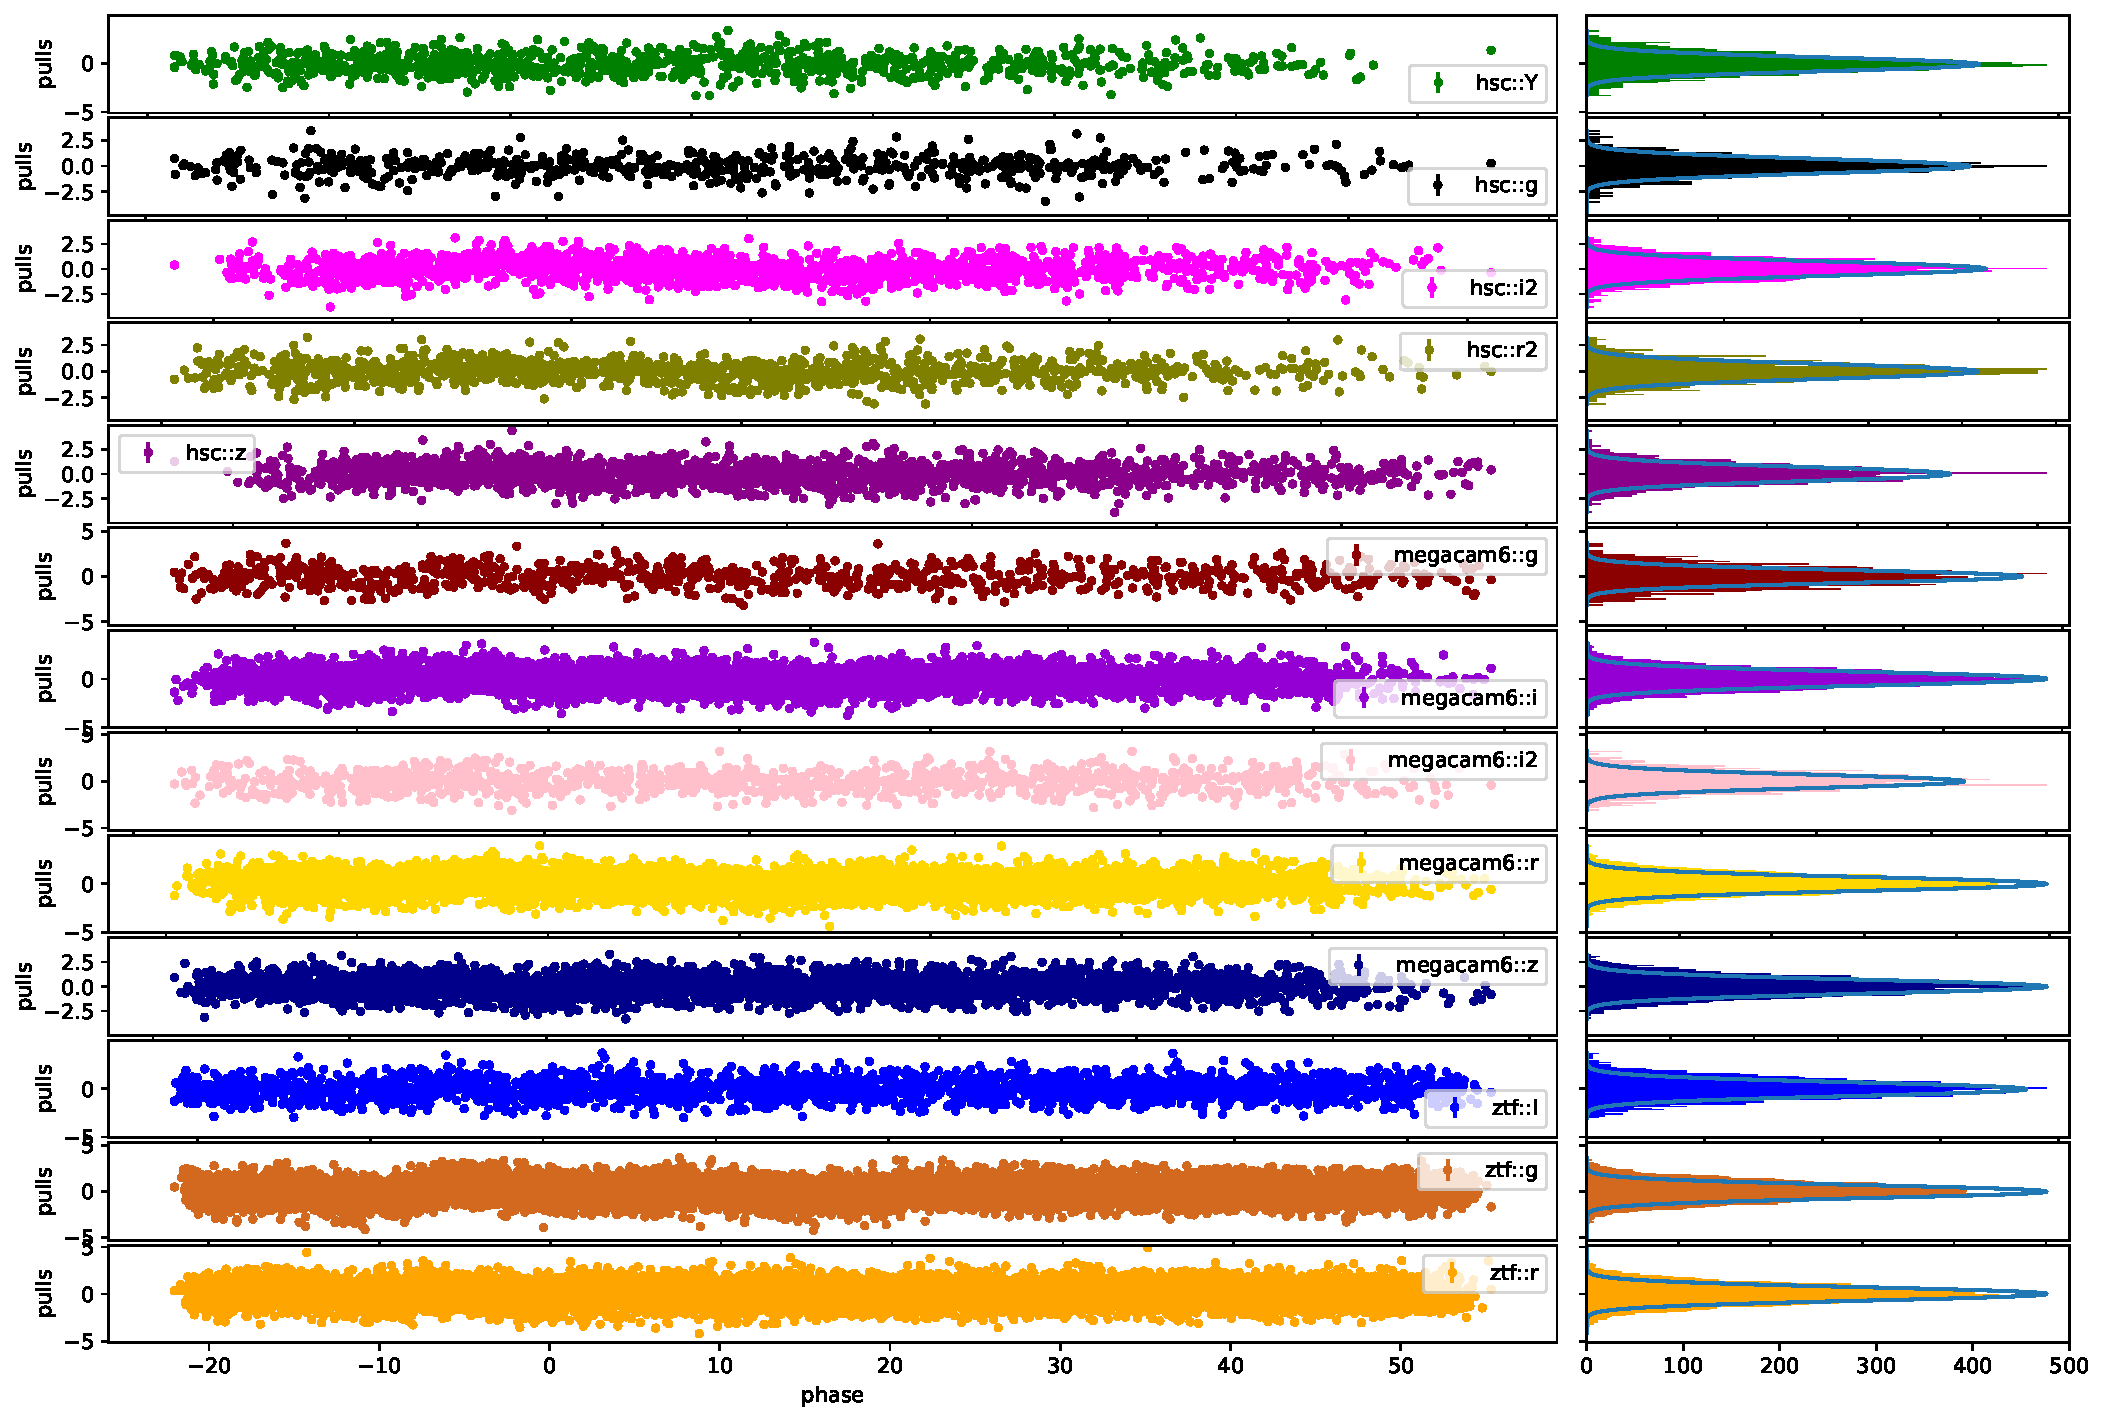
\includegraphics[width=1\textwidth]{MainLayout/DC_chapter/figures/band_resid.pdf}
    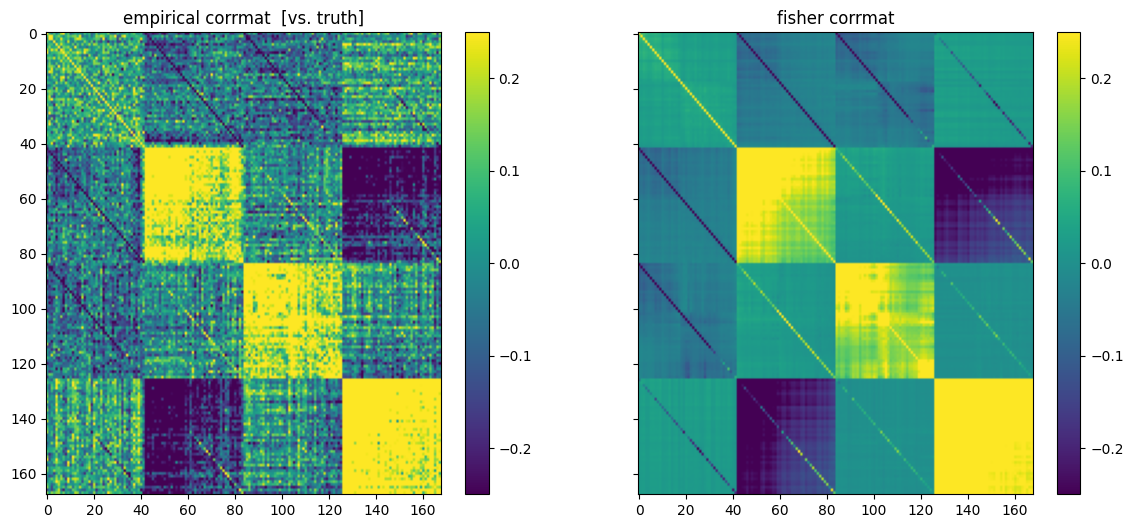
\includegraphics[width=1\textwidth]{MainLayout/DC_chapter/figures/new_fig/corrmats.png}
    \caption{Empirical correlation matrix on the left constructed from the 100 realizations of pre-DC1. Fisher correlation matrix on the right from output of NaCl.}
    \label{fig:pars_corr}
\end{figure}



\subsection{Distance modulus and cosmological parameters reconstruction}

We use EDRIS to determine the distance modulus of the supernovae at the end of the full model training with NaCl. It is important to note
that we are not assessing the efficiency of EDRIS in reconstructing distances as this has already been established in D. Kuhn's 
PhD thesis\footnote{\url{https://theses.hal.science/tel-05451069}} where it was shown that EDRIS does not bias supernova distances in our setup. 
\\

\noindent The results in Figure \ref{fig:pre_dc1_hubble_tot} show the mean binned distance residuals from 100 realizations of pre-DC1 as well as a comparison between
the empirical uncertainties on the binned distances and the Fisher uncertainties from EDRIS. 
We notice significant biases in the mean distance residuals up to $\sim 9$ standard deviations near 
$z \approx 0.1$ and $z \approx 1$, corresponding to the survey 
transition regions between ZTF and SNLS, and at the end of the SNLS and HSC 
surveys. 
The origin of these biases has not yet been conclusively established. 
One possibility is that the model regularization is insufficient, allowing 
artifacts to develop in the reconstructed model and subsequently bias the inferred distances. 
Another possibility is that the quality cuts introduce an effective selection effect. 
Although no explicit selection effects were included in the simulations, these cuts preferentially remove 
some supernovae and may therefore modify the properties of the resulting sample in a way that contributes to the observed bias.\\

\begin{figure}[ht]
    \centering
    %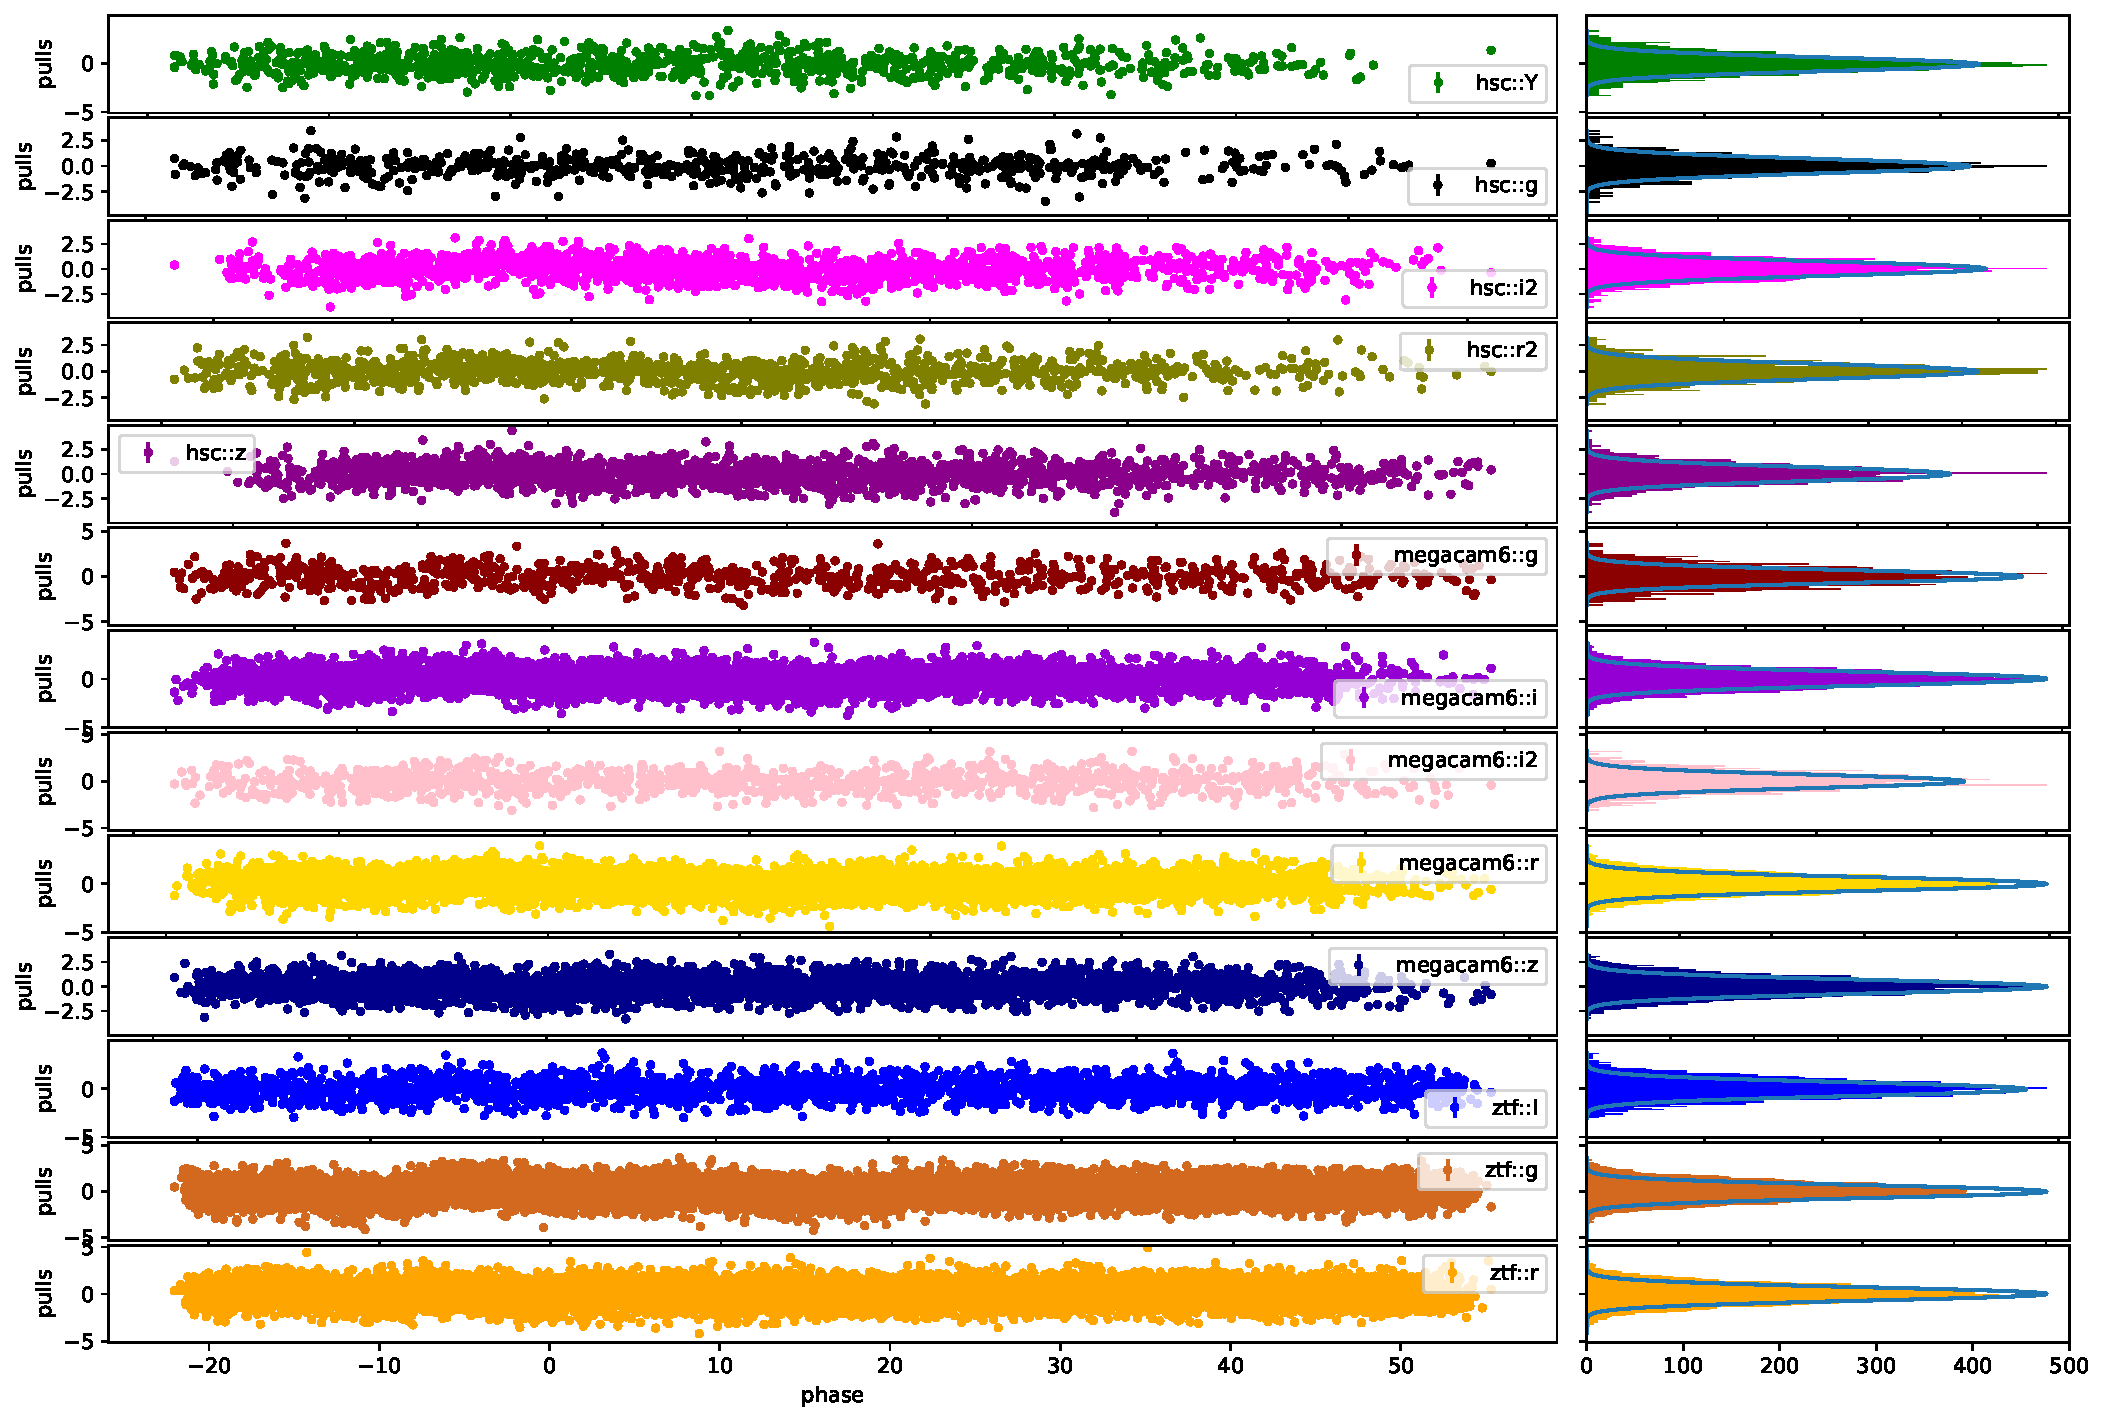
\includegraphics[width=1\textwidth]{MainLayout/DC_chapter/figures/band_resid.pdf}
    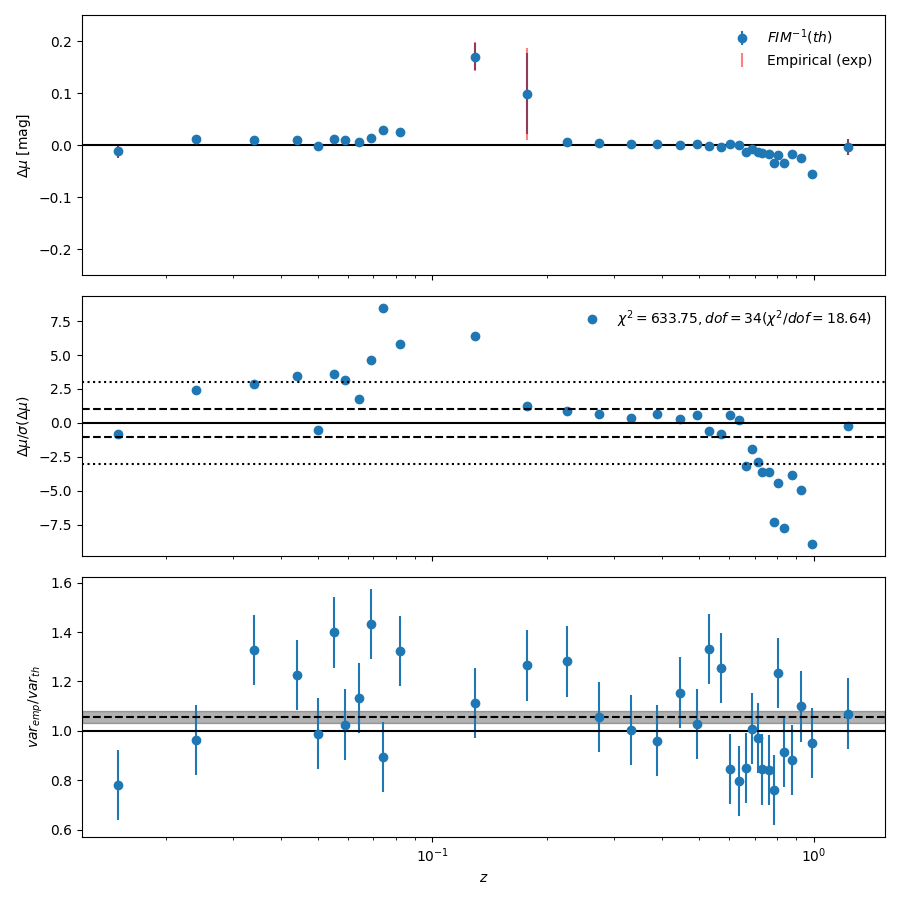
\includegraphics[width=0.8\textwidth]{MainLayout/DC_chapter/figures/new_fig/binned_distances.png}
    \caption{\textit{Top}: Mean of the differences between the reconstructed distance moduli and the truth.
    \textit{Middle}: Weighted residuals of the distance moduli. 
    \textit{Bottom}: Ratio between the empirically constructed variance from EDRIS with the predicted variance. }
    \label{fig:pre_dc1_hubble_tot}
\end{figure}


\noindent 
The \textsc{Lemaître} pipeline outputs constraints on 
$\Omega_{bc} = \Omega_b + \Omega_c$, the combined baryon and cold 
dark matter density parameter. The neutrino mass is fixed to 
its Planck 2018 minimal mass value and the 
neutrino density parameter $\Omega_\nu$ is small compared to $\Omega_{bc}$ (less than 5\% contributtion to $\Omega_m$)
and therefore approximate $\Omega_m \approx \Omega_{bc}$. 
Results from \texttt{cosmologix} are shown in Figure \ref{fig:dc1_contour} where we show the $\Omega_m$-$w$ contours for six randomly selected individual 
realizations of pre-DC1. We see that amongst them are realizations that we recover the input cosmological parameters within 1 standard deviation while others show significant deviations. 
The distribution of the recovered $\Omega_m$-$w$ parameters from the 100 realizations is seen Figure \ref{fig:w_om_dist}. 

Across the 100 realizations, we find strong biases in the recovered cosmological parameters, with the mean values of $\Omega_m$ and $w$ displaced from their input values by
$15.5 \sigma$ and $10.4 \sigma$ respectively. 
This bias persists when fixing  $w=-1$ and fitting only for $\Omega_m$ for which the recovered mean is displaced from the input value by $19.4 \sigma$ as seen in Figure \ref{fig:om_dist}.
The origin of this bias is currently unknown, but it is likely related to the biases identified in the reconstructed distance moduli, 
since the cosmological parameters are inferred from these distances. \\

\begin{figure}[ht]
    \centering
    %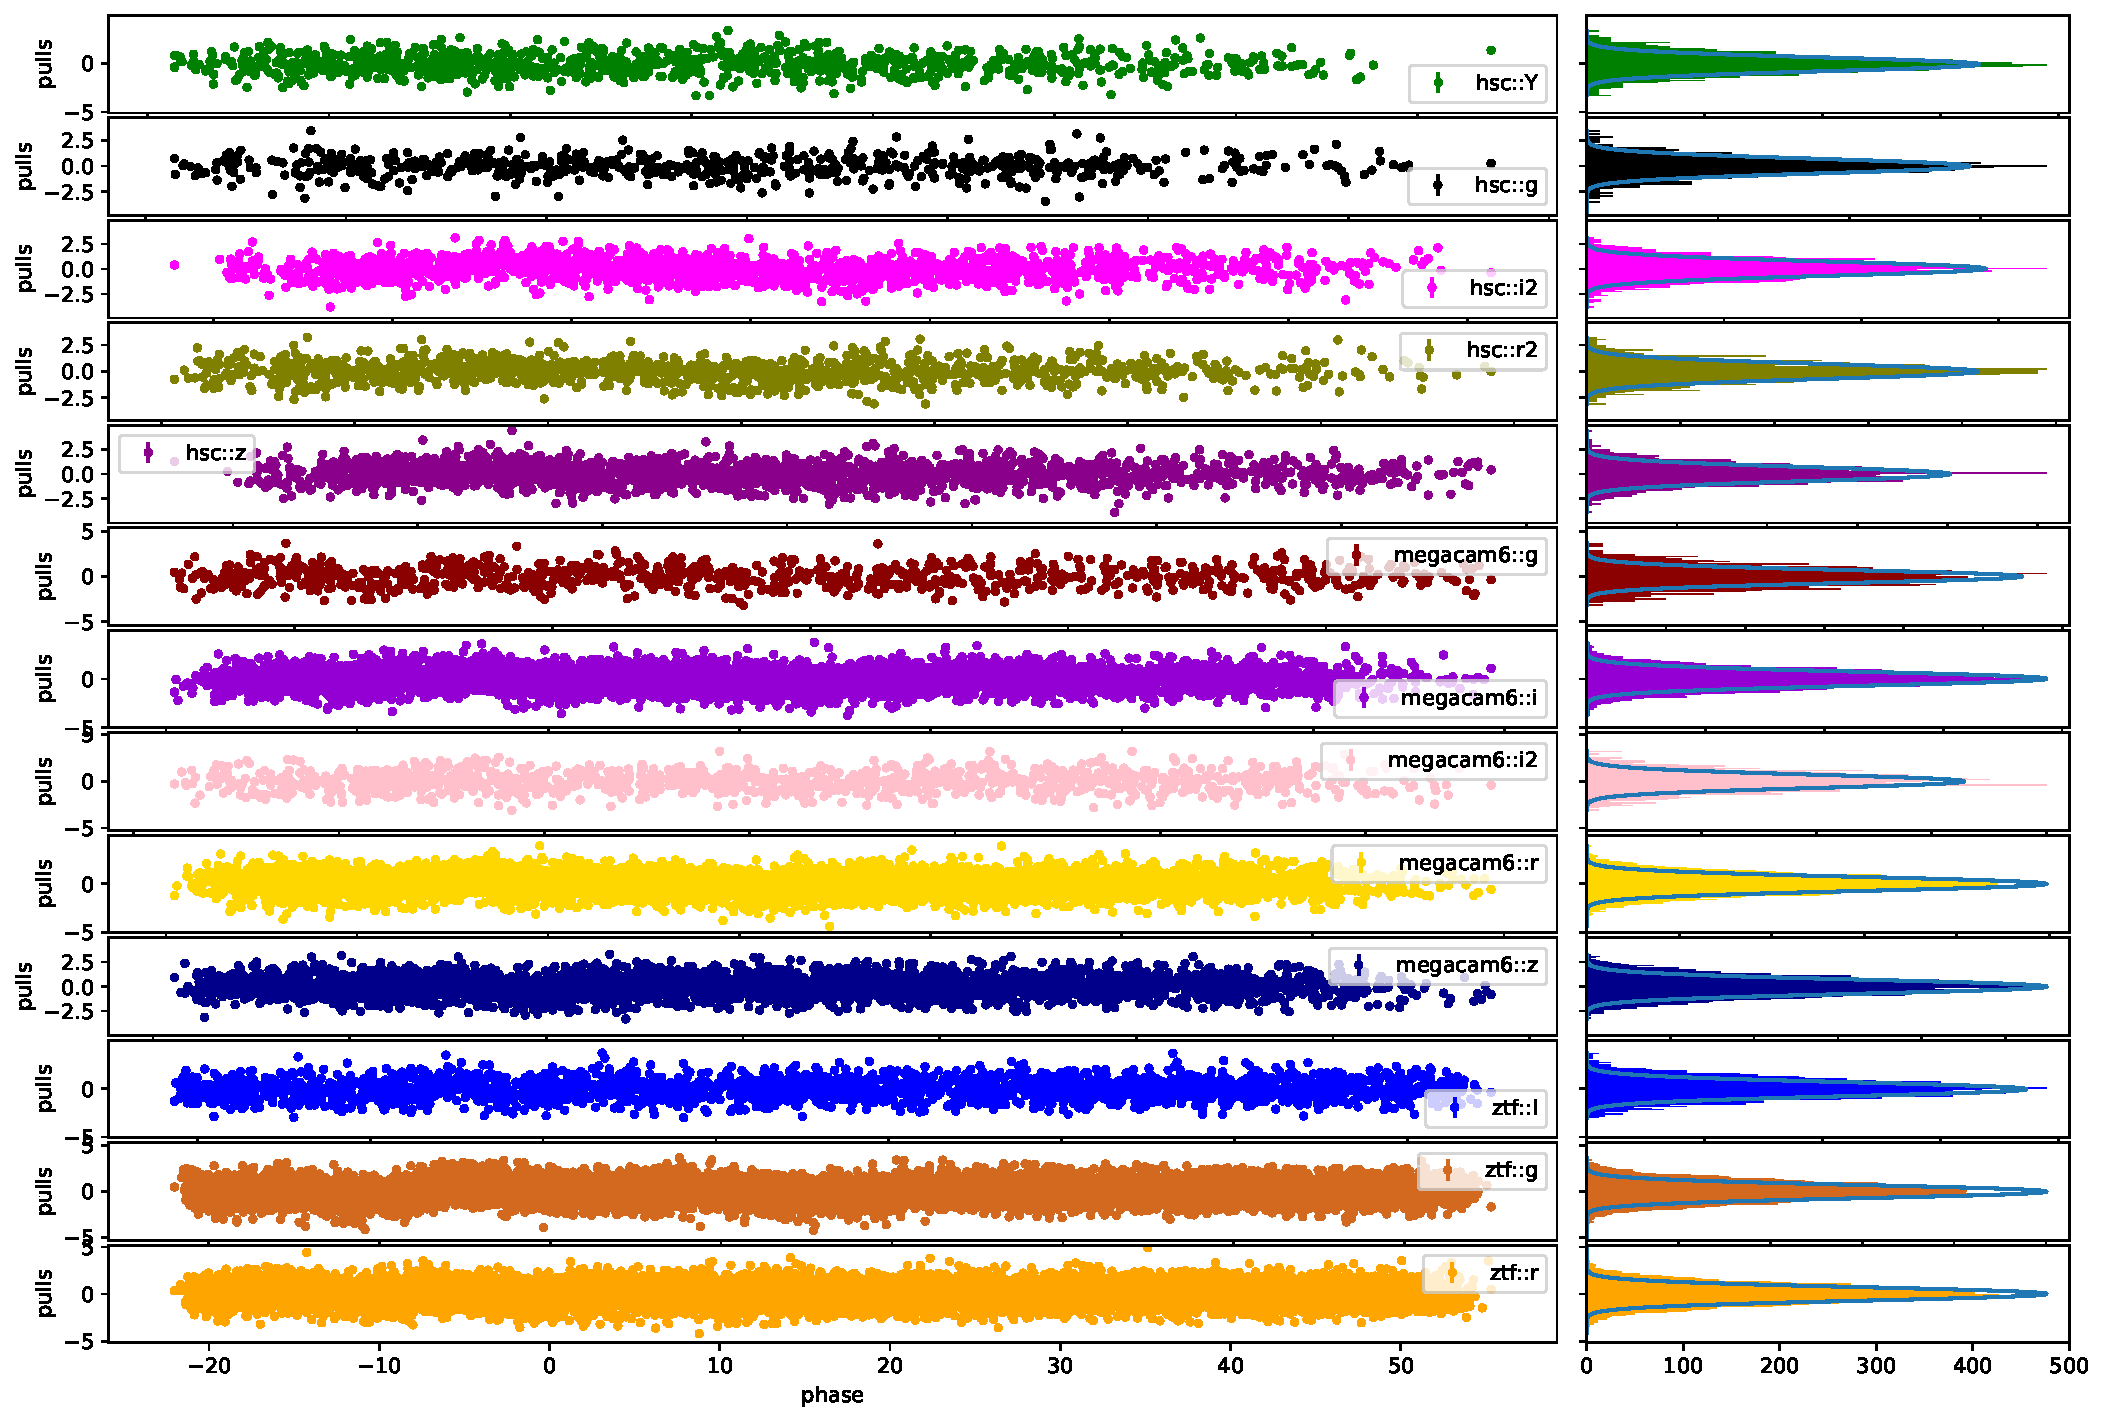
\includegraphics[width=1\textwidth]{MainLayout/DC_chapter/figures/band_resid.pdf}
    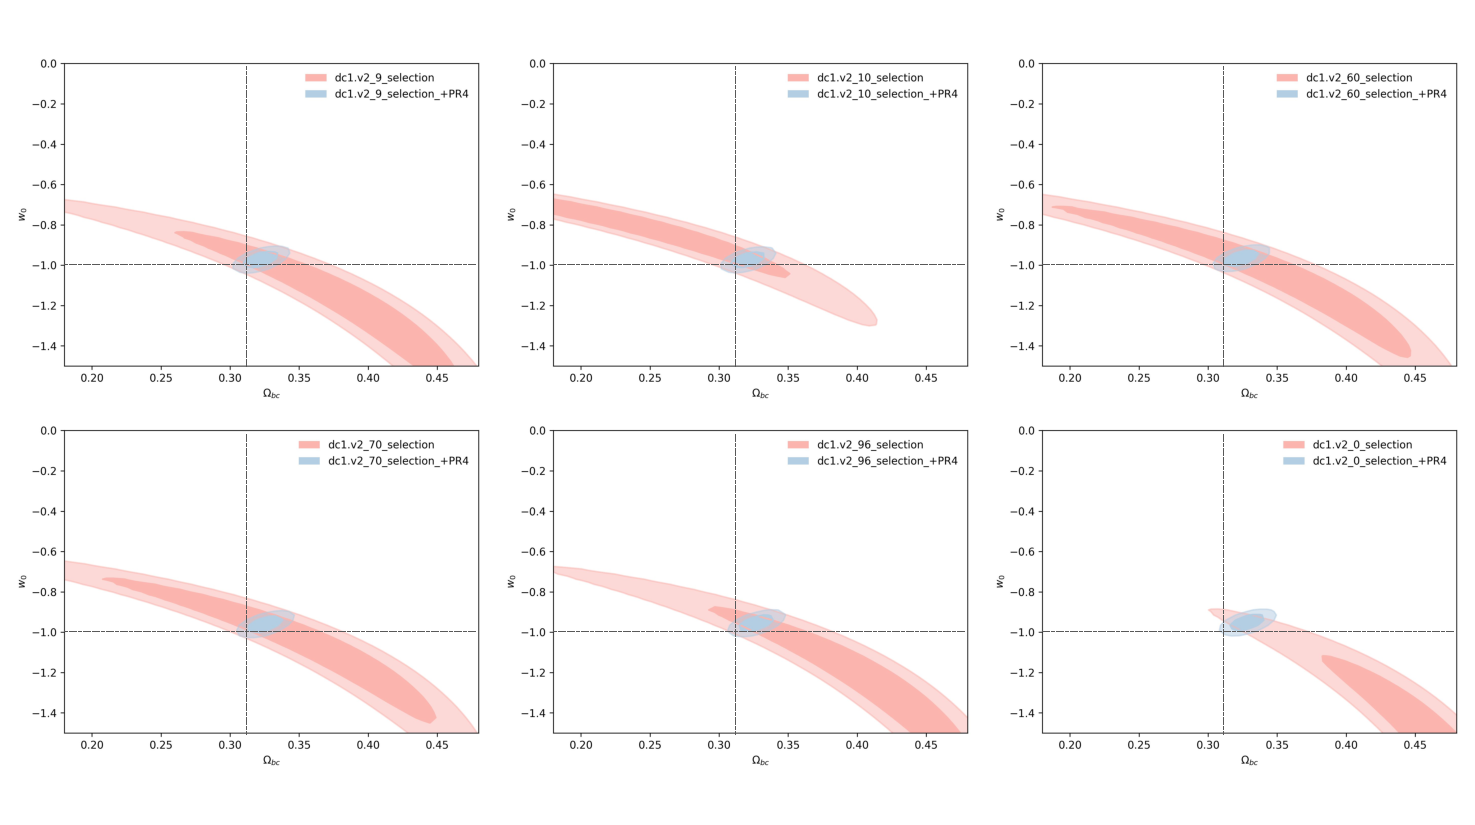
\includegraphics[width=1\textwidth]{MainLayout/DC_chapter/figures/new_fig/contour_comp.pdf}
    \caption{$\Omega_m$-$w$ contours for six realizations of pre-DC1 in the red area. The blue area shows the constraining power when coupled with Planck CMB results.}
    \label{fig:dc1_contour}
\end{figure}

\begin{figure}[ht]
    \centering
    %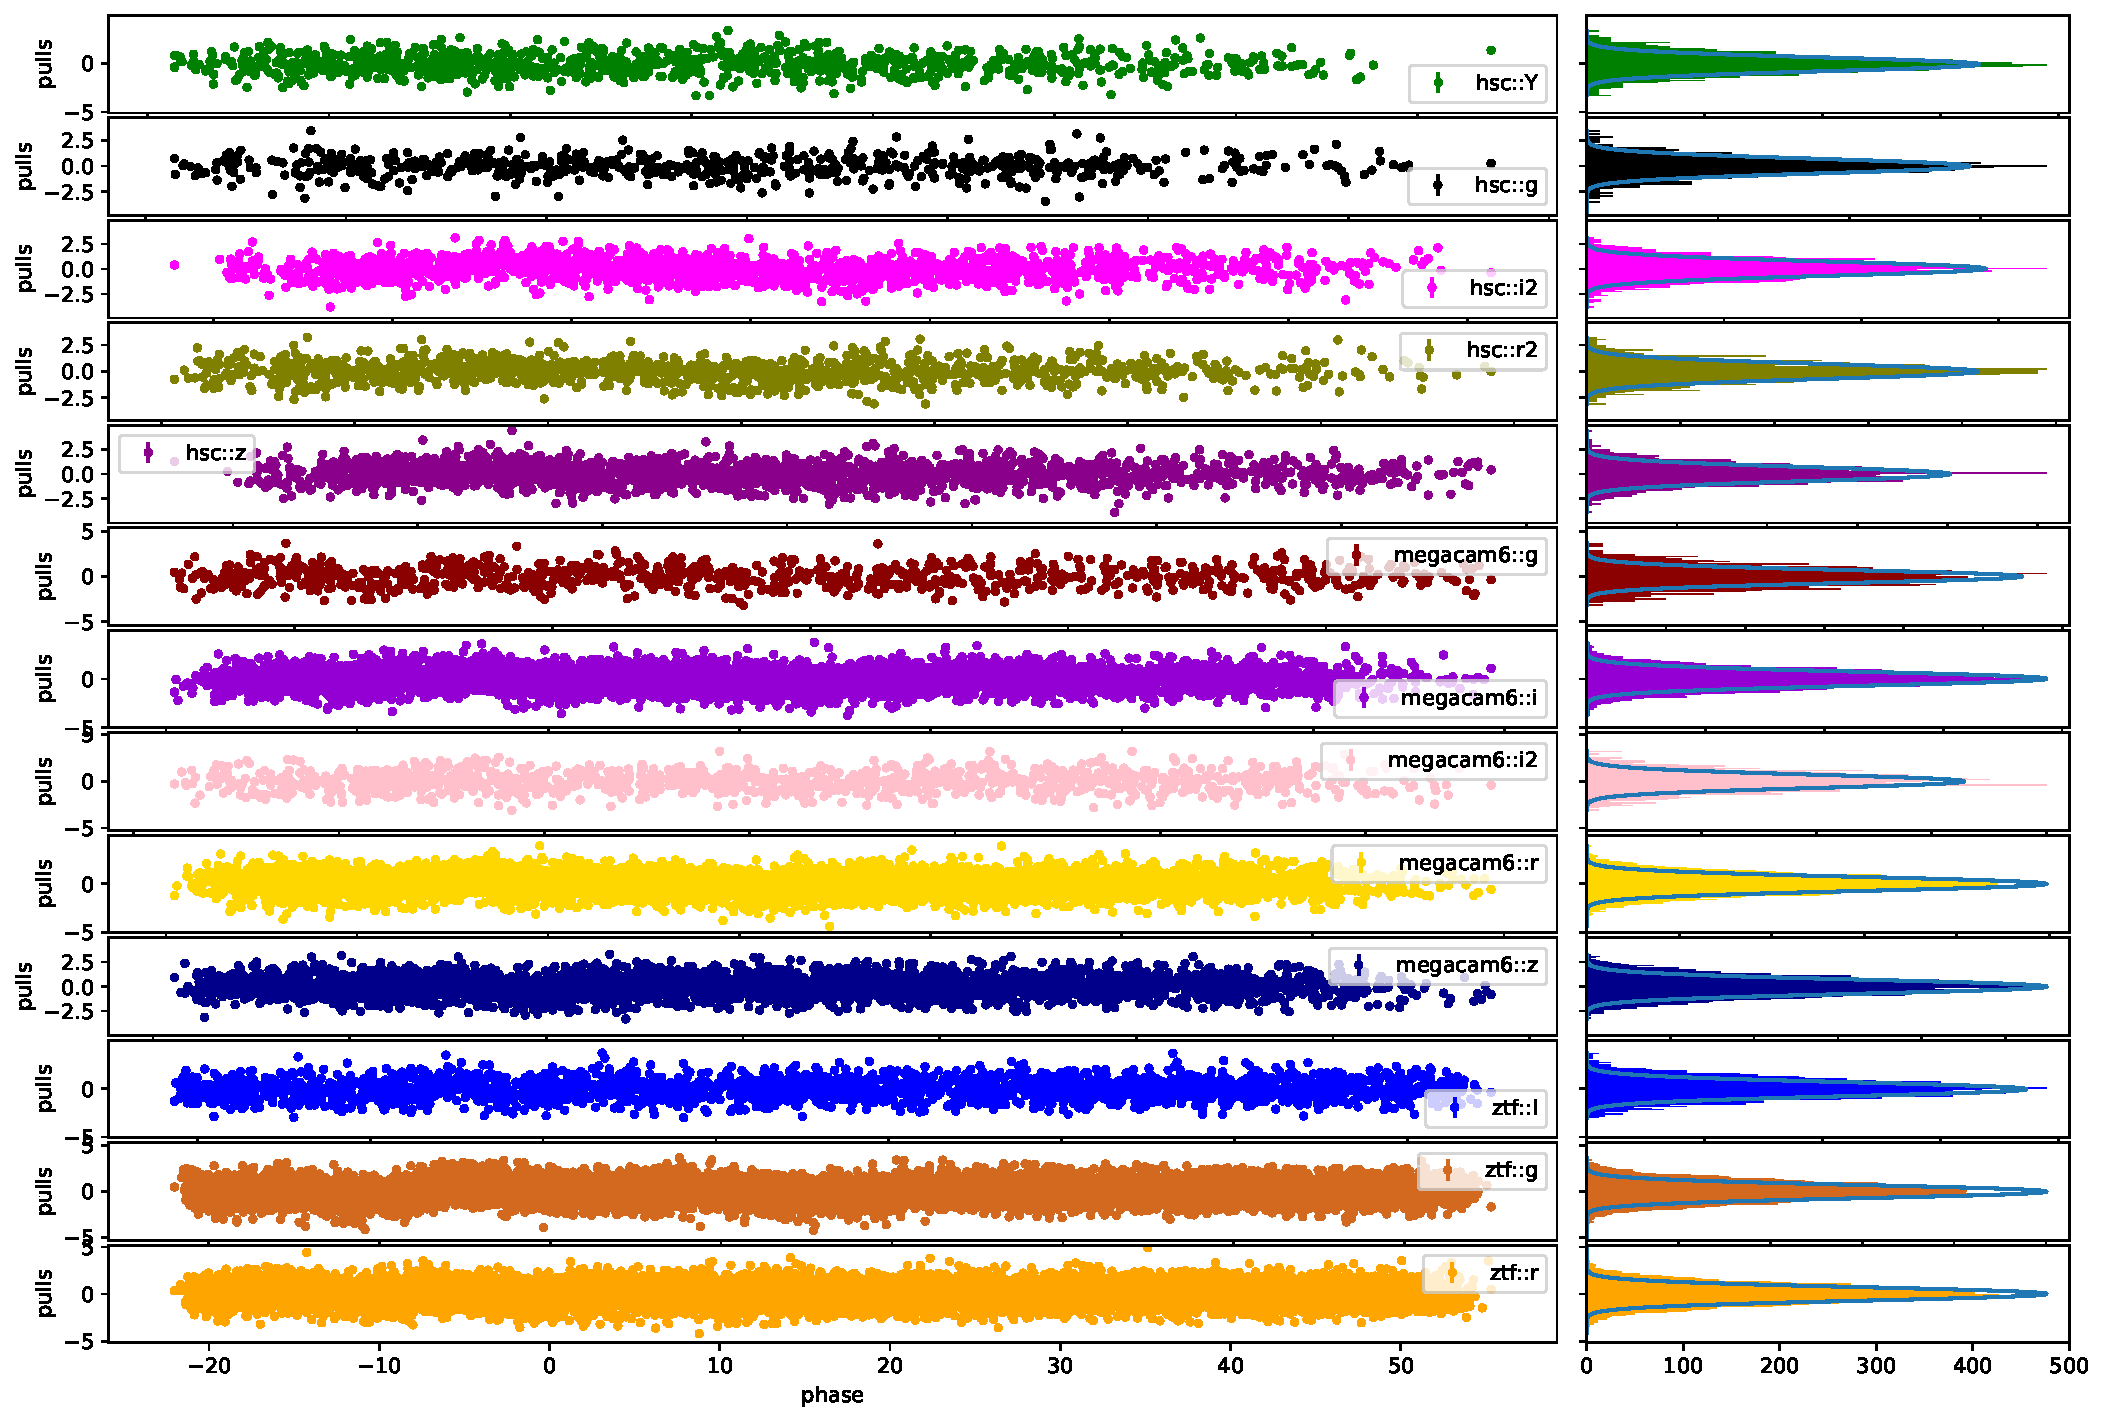
\includegraphics[width=1\textwidth]{MainLayout/DC_chapter/figures/band_resid.pdf}
    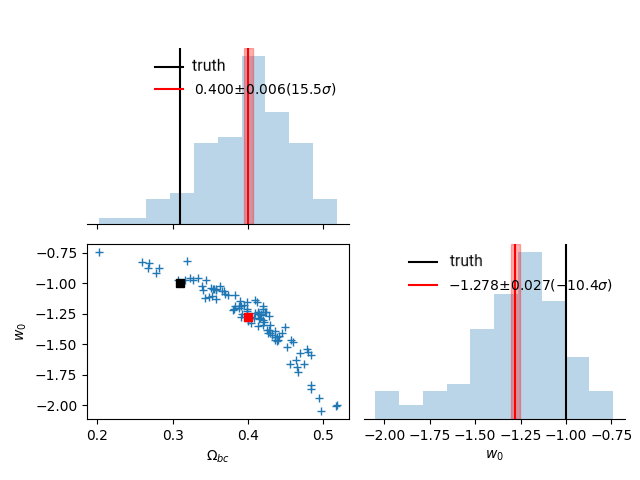
\includegraphics[width=0.8\textwidth]{MainLayout/DC_chapter/figures/new_fig/fwcdm.png}
    \caption{Distribution of $\Omega_m$ and $w$ for the 100 realizations of pre-DC1. The red line represents the mean value of each cosmological parameter as well its 
    standard deviation. The black line represents the expected results used as input for the simulation.}
    \label{fig:w_om_dist}
\end{figure}

\begin{figure}[ht]
    \centering
    %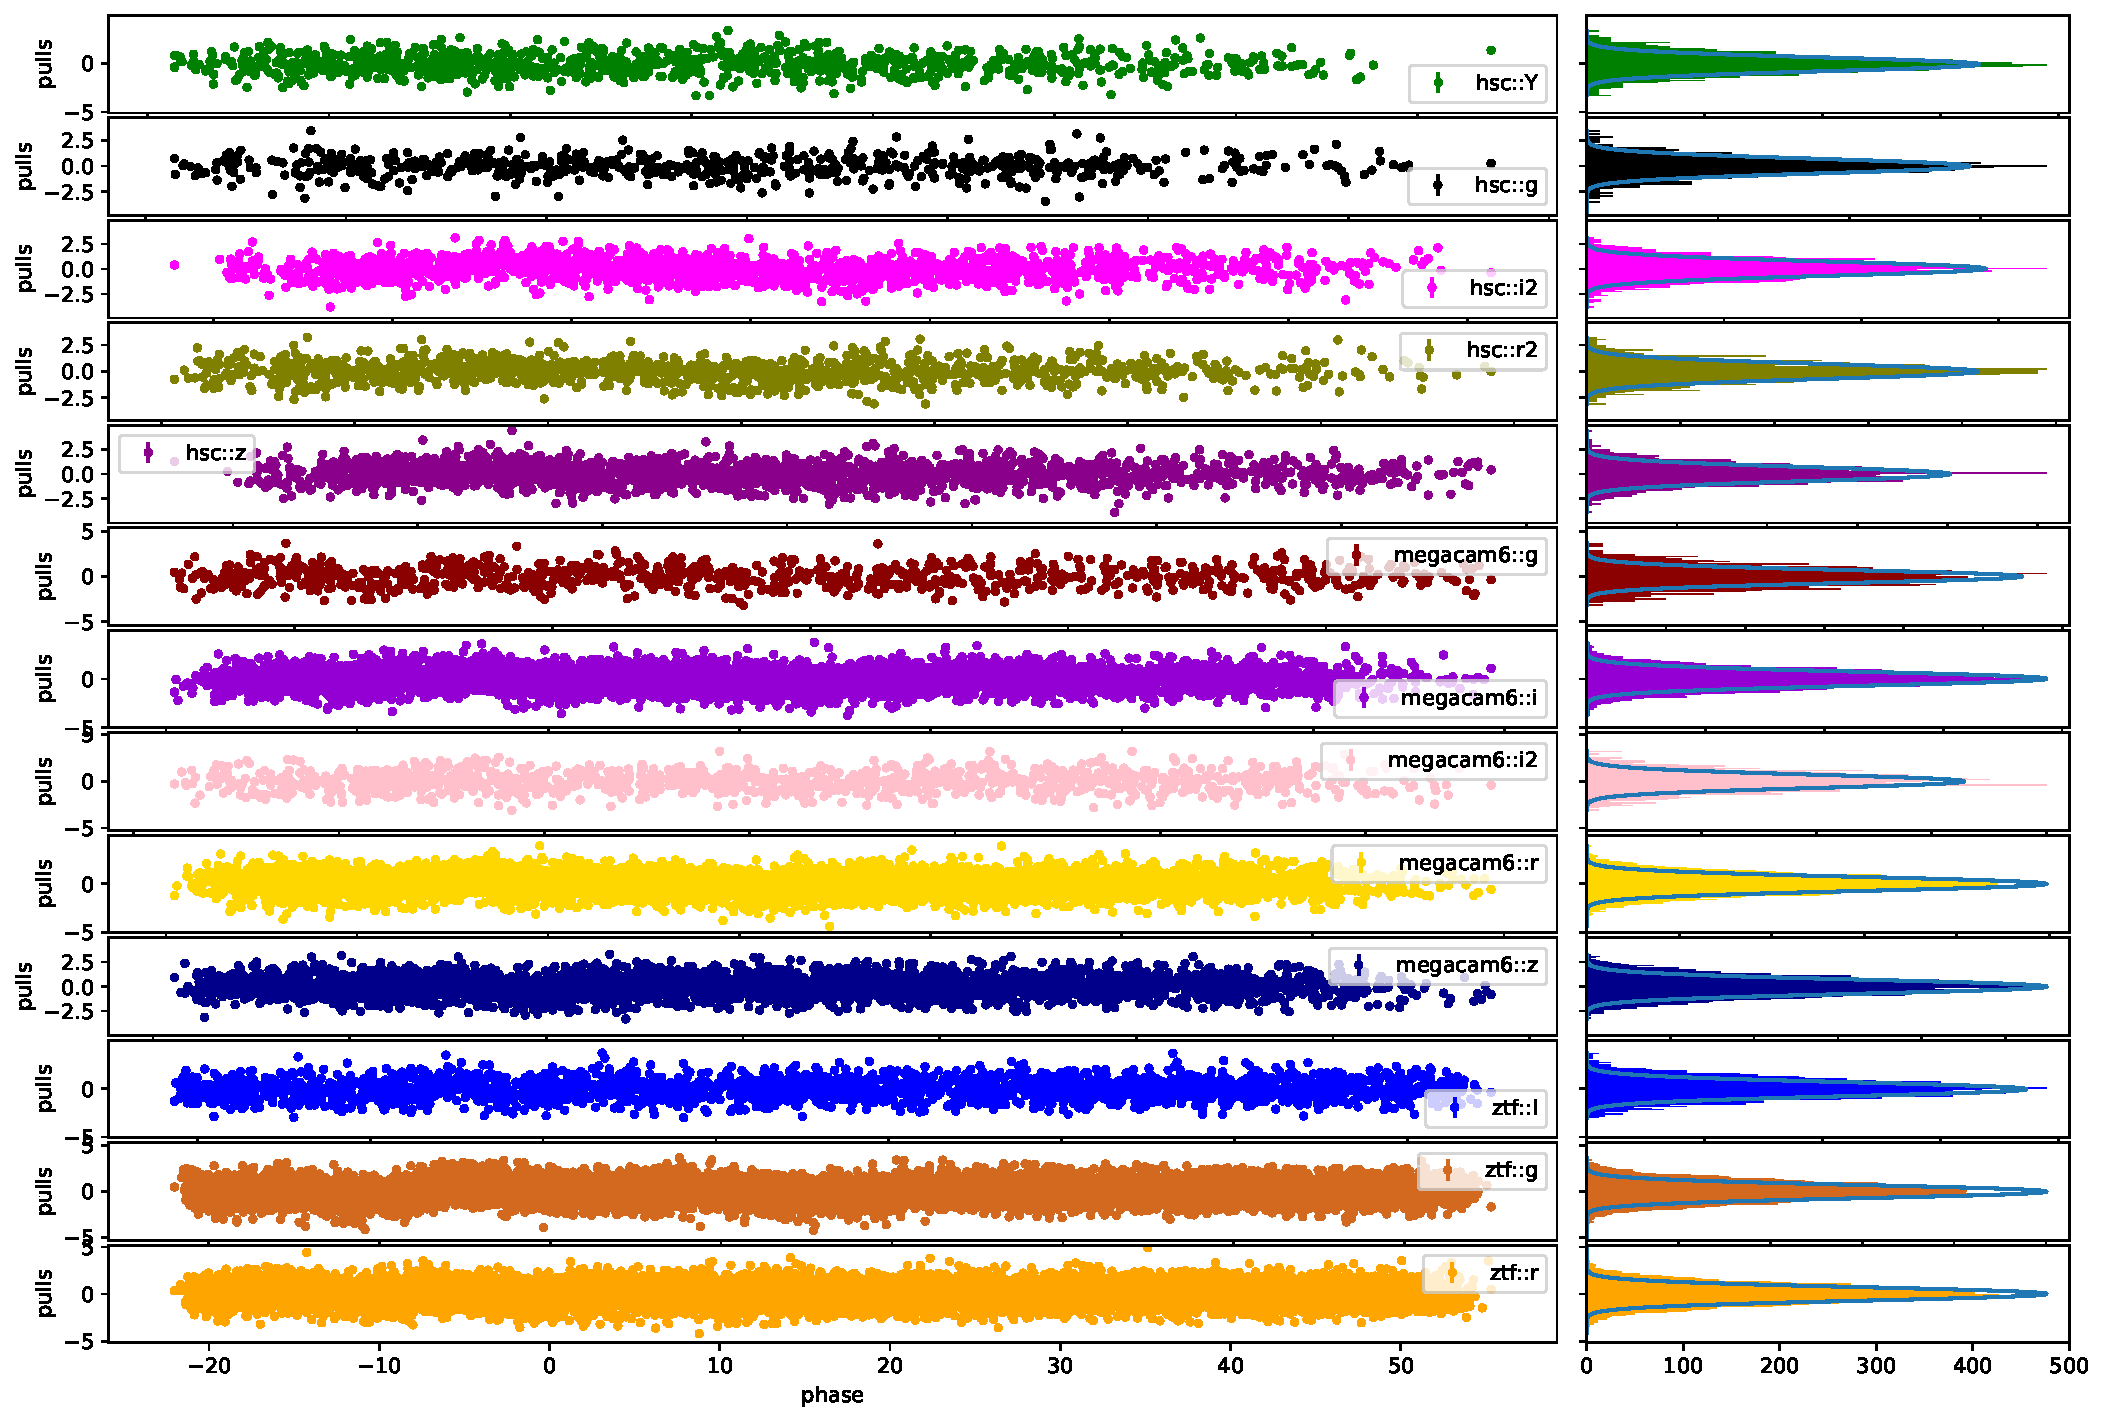
\includegraphics[width=1\textwidth]{MainLayout/DC_chapter/figures/band_resid.pdf}
    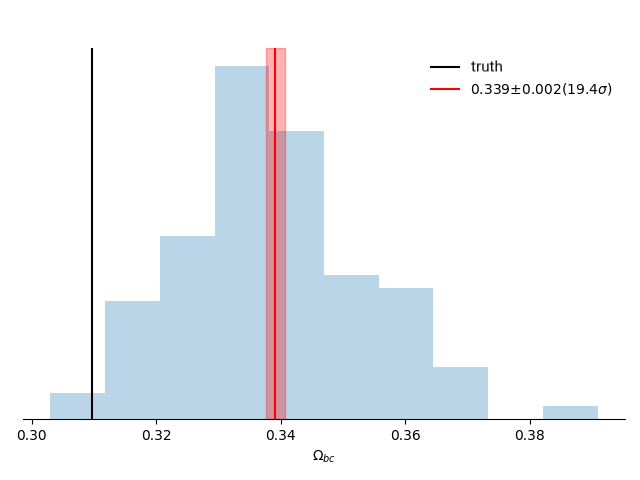
\includegraphics[width=0.6\textwidth]{MainLayout/DC_chapter/figures/new_fig/flcdm.png}
    \caption{Distribution of $\Omega_m$ for a fixed value of $w=-1$. 
    The red line represents the mean value the recovered $\Omega_m$ as well its 
    standard deviation. The black line represents the expected results used as input for the simulation.}
    \label{fig:om_dist}
\end{figure}

\section{Conclusion}

This chapter presented the first application of the NaCl framework
to real data on the SNfactory dataset and 
to simulated \textsc{Lemaître}-like datasets through the pre-DC1 
validation programme. The results demonstrate that NaCl accurately 
describes the spectrophotometric evolution of Type Ia supernovae and 
that its Fisher uncertainty estimates are consistent with the empirical uncertainties for the large majority of parameters, with a small overestimate in the empirical 
uncertainties that is consistent with finite-sample noise. However, 
significant biases were identified in the reconstructed distance 
moduli near the survey transition redshifts $z \approx 0.1$ and 
$z \approx 1$, which likely propagate into the cosmological parameter 
inference as biases in both $\Omega_m$ and $w$. 
The origin 
of these biases has not yet been conclusively identified, with 
possible contributions from residual model artifacts associated with 
the regularization and effective selection effects introduced by the 
quality cuts. 
Resolving these 
biases is the primary objective before the pipeline can be applied to the blinded 
\textsc{Lemaître} dataset. Accurate distance measurements are 
also of significant importance for the $f\sigma_8$ analysis, making this 
validation work directly relevant to both the dark energy and 
growth rate science goals of the \textsc{Lemaître} project.


%\begin{figure}[ht]
%    \centering
    %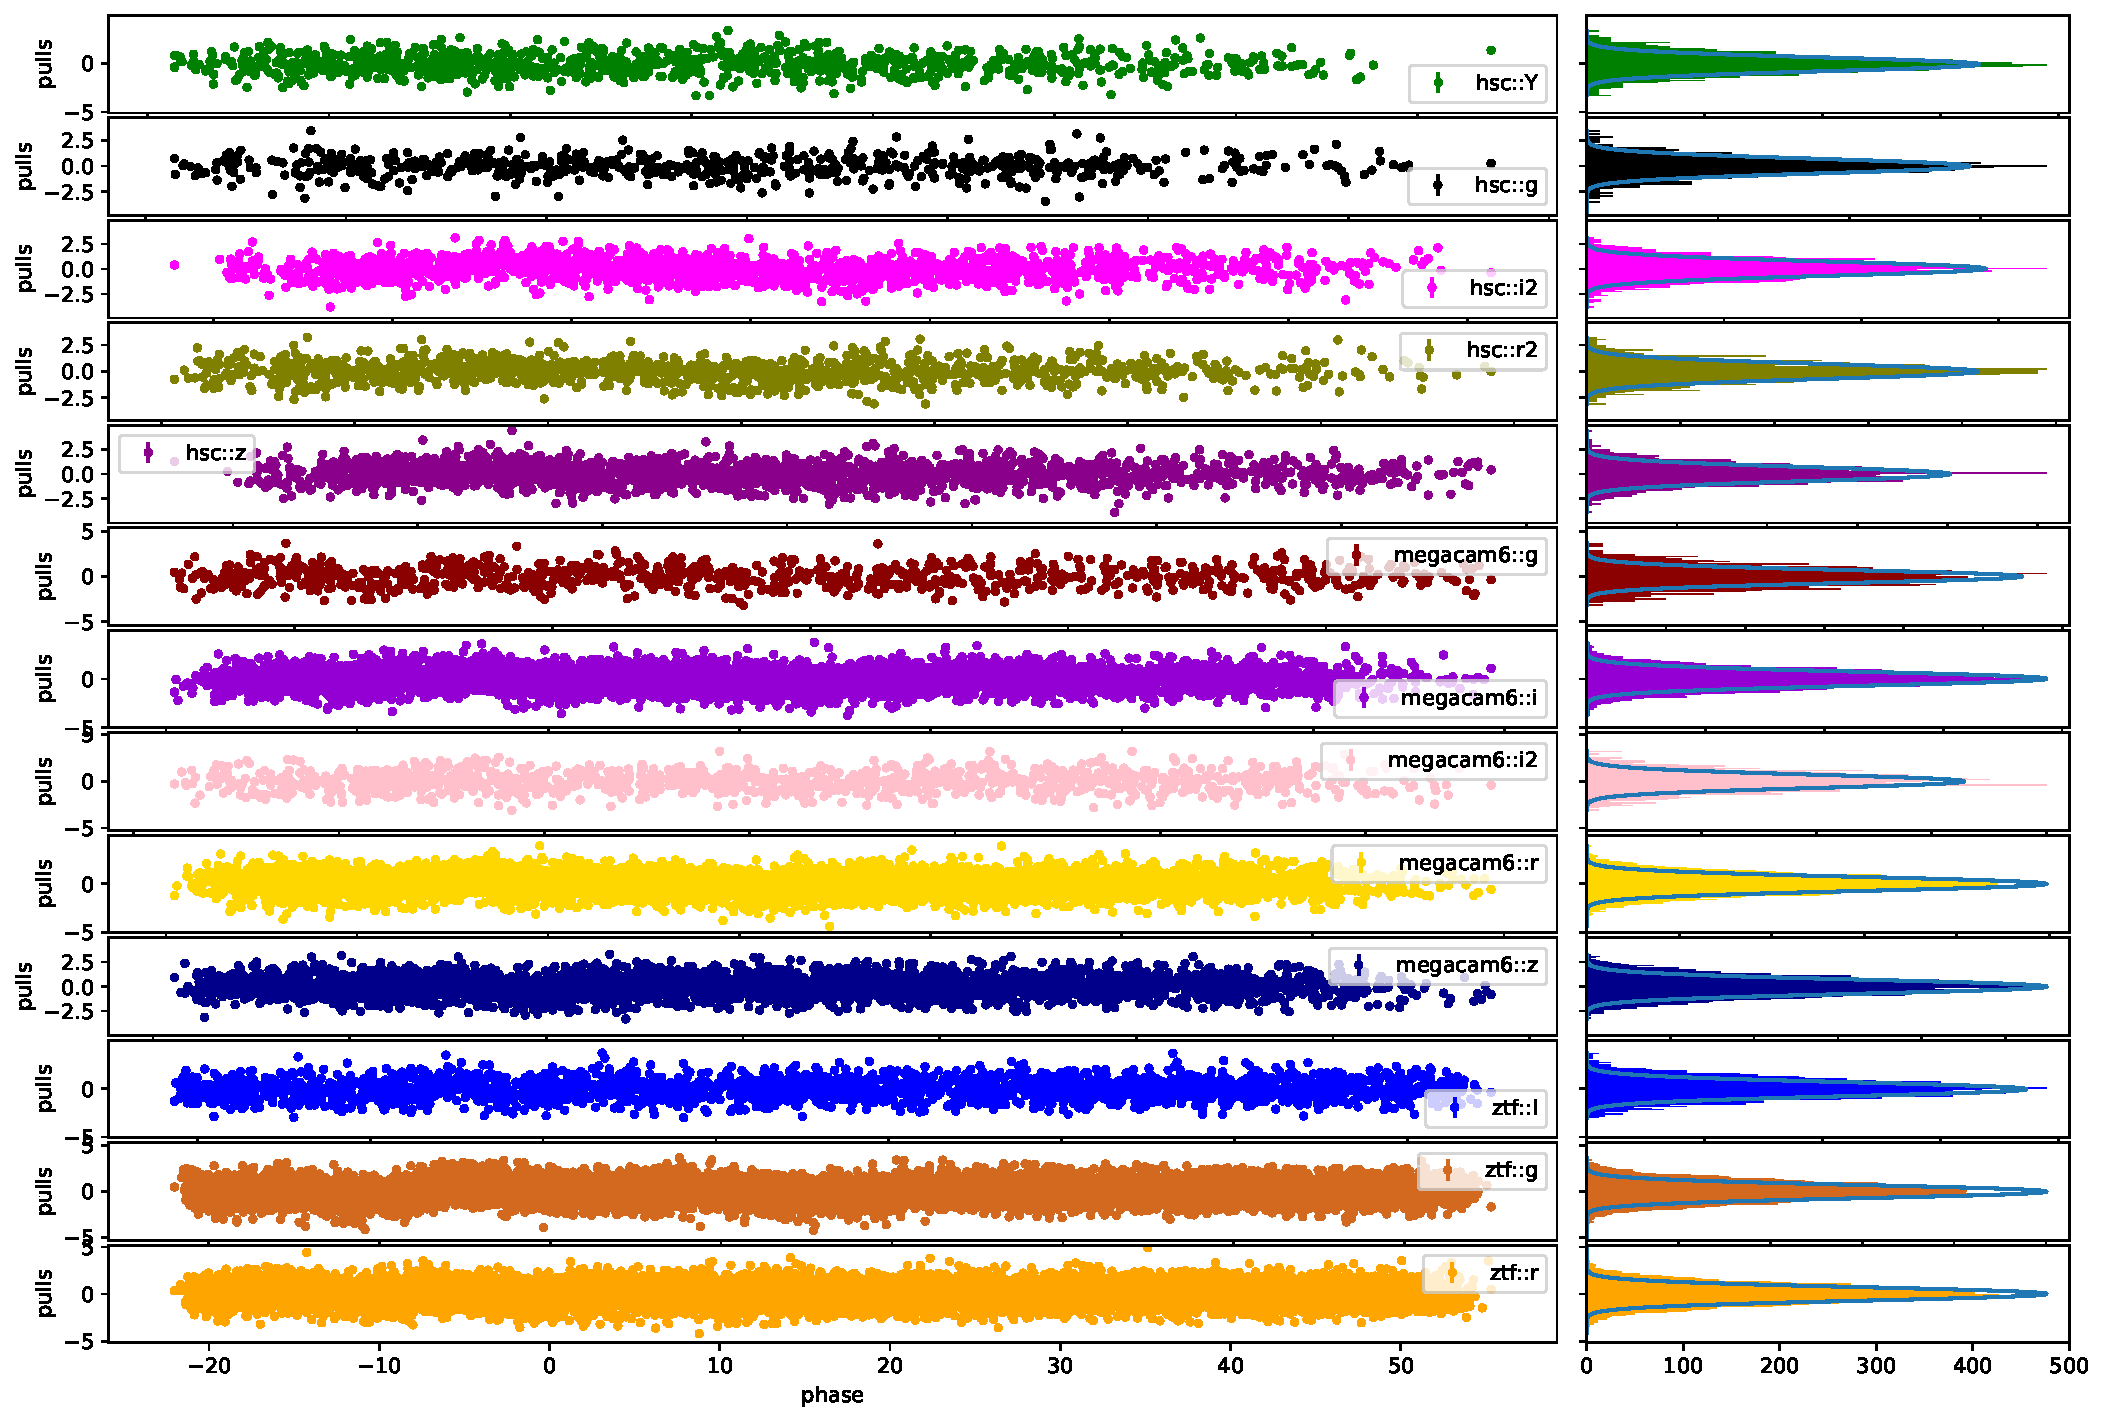
\includegraphics[width=1\textwidth]{MainLayout/DC_chapter/figures/band_resid.pdf}
%    \includegraphics[width=0.8\textwidth]{MainLayout/DC_chapter/figures/None}
%    \caption{$\Omega_m$ and $w$ coverage for 100 realization of pre-DC1}
%    \label{fig:dc1_om_w_coverage}
%\end{figure}
